% Práctica 2: Ontologías - Fundamentos de Inteligencia Artificial
% Master en Inteligencia Artificial 2025-26
% Santiago Delgado Ferreiro & David Carballo Rodríguez

\documentclass[12pt,a4paper]{article}

% Paquetes esenciales
\usepackage[utf8]{inputenc}
\usepackage[spanish]{babel}
\usepackage{graphicx}
\usepackage{float}
\usepackage{hyperref}
\usepackage{listings}
\usepackage{xcolor}
\usepackage{geometry}
\usepackage{fancyhdr}
\usepackage{titlesec}
\usepackage{enumitem}
\usepackage{caption}
\usepackage{subcaption}

% Configuración de página
\geometry{
    top=2.5cm,
    bottom=2.5cm,
    left=3cm,
    right=3cm
}

% Configuración de encabezados y pies de página
\pagestyle{fancy}
\fancyhf{}
\fancyhead[L]{Práctica 2: Ontologías}
\fancyhead[R]{AIF 2025-26}
\fancyfoot[C]{\thepage}
\renewcommand{\headrulewidth}{0.4pt}
\renewcommand{\footrulewidth}{0.4pt}

% Configuración de hipervínculos
\hypersetup{
    colorlinks=true,
    linkcolor=blue,
    filecolor=magenta,      
    urlcolor=cyan,
    pdftitle={Práctica 2: Ontologías},
    pdfauthor={Santiago Delgado Ferreiro, David Carballo Rodríguez},
}

% Configuración de listados de código
\lstdefinelanguage{SPARQL}{
    keywords={PREFIX, SELECT, WHERE, FILTER, OPTIONAL, UNION, GROUP, ORDER, BY, LIMIT, DISTINCT, COUNT, YEAR, ASC},
    keywordstyle=\color{blue}\bfseries,
    string=[s]{"}{"},
    stringstyle=\color{red},
    comment=[l]{\#},
    commentstyle=\color{gray}\itshape,
    morecomment=[s]{/*}{*/},
    sensitive=true,
    basicstyle=\ttfamily\small,
    breaklines=true,
    showstringspaces=false,
    frame=single,
    numbers=left,
    numberstyle=\tiny\color{gray},
    numbersep=5pt,
}

\lstset{
    basicstyle=\ttfamily\small,
    breaklines=true,
    frame=single,
    numbers=left,
    numberstyle=\tiny\color{gray},
}

% Título personalizado
\title{
    \vspace{-2cm}
    \includegraphics[width=0.3\textwidth]{logo_universidad.png}\\ % Añadir logo si está disponible
    \vspace{1cm}
    \textbf{Fundamentos de Inteligencia Artificial}\\
    \Large Práctica 2: Ontologías\\
    \large Master en Inteligencia Artificial\\
    \normalsize Curso Académico 2025-26
}

\author{
    Santiago Delgado Ferreiro\\
    \texttt{santiago.delgado@estudiante.uam.es}
    \and
    David Carballo Rodríguez\\
    \texttt{david.carballo@estudiante.uam.es}
}

\date{27 de Octubre de 2025}

\begin{document}

% Portada
\maketitle
\thispagestyle{empty}

\vfill

\begin{center}
\textbf{Grupo de Prácticas:} [Completar número de grupo]\\
\vspace{0.5cm}
\textbf{Username WebProtégé:} santi\_david
\end{center}

\newpage

% Índice
\tableofcontents
\newpage

% Configurar numeración de páginas
\setcounter{page}{1}

%==============================================================================
% SECCIÓN 1: INTRODUCCIÓN
%==============================================================================
\section{Introducción}

Las ontologías son representaciones formales del conocimiento que permiten estructurar y organizar información de manera semántica. En el contexto de la Inteligencia Artificial, las ontologías juegan un papel fundamental al proporcionar:

\begin{itemize}
    \item \textbf{Representación del conocimiento:} Estructuración formal de conceptos y sus relaciones.
    \item \textbf{Interoperabilidad:} Facilitan el intercambio de información entre sistemas heterogéneos.
    \item \textbf{Razonamiento automático:} Permiten inferir nuevo conocimiento a partir de hechos existentes.
    \item \textbf{Reutilización del conocimiento:} Promueven la creación de bases de conocimiento compartidas.
\end{itemize}

\subsection{Objetivos de la Práctica}

Los objetivos principales de esta práctica son:

\begin{enumerate}
    \item \textbf{Comprender la estructura de ontologías} mediante el análisis de la ontología OFFF (Ontology of Fast Food Facts).
    \item \textbf{Editar ontologías} utilizando la herramienta WebProtégé, añadiendo clases, propiedades e instancias.
    \item \textbf{Realizar consultas SPARQL} sobre bases de conocimiento disponibles en la Web Semántica (DBpedia).
    \item \textbf{Aplicar conocimientos teóricos} a casos prácticos relacionados con la nutrición y salud alimentaria.
\end{enumerate}

\subsection{Herramientas Utilizadas}

\begin{itemize}
    \item \textbf{WebProtégé:} Editor colaborativo de ontologías basado en web (\url{https://webprotege.stanford.edu/})
    \item \textbf{OFFF:} Ontología de comida rápida que integra información nutricional
    \item \textbf{SPARQL:} Lenguaje de consulta para datos RDF
    \item \textbf{DBpedia:} Base de conocimiento extraída de Wikipedia
\end{itemize}

%==============================================================================
% SECCIÓN 2: EDICIÓN DE ONTOLOGÍA OFFF
%==============================================================================
\section{Edición de Ontología OFFF}

\subsection{Contexto: La Ontología OFFF}

La Ontología de Fast Food Facts (OFFF) es una representación formal del conocimiento sobre comida rápida, desarrollada por UTHealth. Esta ontología integra:

\begin{itemize}
    \item Información nutricional de productos de comida rápida
    \item Componentes alimentarios (carbohidratos, proteínas, grasas, vitaminas, minerales)
    \item Alérgenos presentes en los alimentos
    \item Ingredientes específicos
    \item Relaciones con resultados de salud (health outcomes)
\end{itemize}

La estructura jerárquica de OFFF permite establecer relaciones causales entre la calidad de la dieta y diversos problemas de salud, facilitando el análisis y razonamiento sobre hábitos alimentarios.

\subsection{Selección de Alérgenos}

Para esta práctica se han seleccionado 10 alérgenos de la lista oficial de alérgenos alimentarios reconocidos internacionalmente (\url{https://en.wikipedia.org/wiki/List_of_allergens}). La selección se ha basado en los siguientes criterios:

\begin{enumerate}
    \item \textbf{Prevalencia:} Alérgenos más comunes en la población general
    \item \textbf{Severidad:} Potencial de causar reacciones alérgicas graves
    \item \textbf{Regulación:} Obligatoriedad de etiquetado en múltiples jurisdicciones
    \item \textbf{Presencia en comida rápida:} Frecuencia de aparición en productos de fast food
\end{enumerate}

\subsubsection{Alérgenos Seleccionados}

\begin{enumerate}
    \item \textbf{Peanut (Cacahuete)}
    \begin{itemize}
        \item Uno de los alérgenos más comunes y potencialmente mortales
        \item Presente en aceites, salsas y productos procesados
        \item Causa reacciones anafilácticas en individuos sensibles
    \end{itemize}
    
    \item \textbf{Tree Nuts (Frutos secos de árbol)}
    \begin{itemize}
        \item Incluye almendras, nueces, avellanas, anacardos, pistachos
        \item Frecuente en ensaladas, postres y productos horneados
        \item Alto riesgo de reacciones cruzadas entre diferentes frutos secos
    \end{itemize}
    
    \item \textbf{Milk (Leche)}
    \begin{itemize}
        \item Alérgeno más común en niños pequeños
        \item Presente en lácteos, helados, salsas cremosas, productos horneados
        \item Diferentes de la intolerancia a la lactosa
    \end{itemize}
    
    \item \textbf{Egg (Huevo)}
    \begin{itemize}
        \item Especialmente la clara de huevo (albúmina)
        \item Usado en mayonesas, productos horneados, empanados
        \item Común en productos de desayuno de comida rápida
    \end{itemize}
    
    \item \textbf{Fish (Pescado)}
    \begin{itemize}
        \item Incluye todos los peces con aletas
        \item Presente en sándwiches de pescado, ensaladas, salsas
        \item Las reacciones suelen persistir toda la vida
    \end{itemize}
    
    \item \textbf{Shellfish (Mariscos)}
    \begin{itemize}
        \item Incluye crustáceos (camarones, cangrejos, langostas) y moluscos
        \item Frecuente en ensaladas, wraps, opciones ``premium''
        \item Una de las alergias más comunes en adultos
    \end{itemize}
    
    \item \textbf{Soy (Soja)}
    \begin{itemize}
        \item Presente en proteínas vegetales, aceites, lecitina
        \item Usado extensivamente en productos procesados
        \item Componente común en hamburguesas vegetarianas
    \end{itemize}
    
    \item \textbf{Wheat (Trigo)}
    \begin{itemize}
        \item Contiene gluten (proteína causante de alergias)
        \item Presente en panes, masas, empanados, espesantes
        \item Diferente de la enfermedad celíaca
    \end{itemize}
    
    \item \textbf{Sesame (Sésamo)}
    \begin{itemize}
        \item Cada vez más reconocido como alérgeno importante
        \item Presente en panes (panecillos), salsas (tahini), aceites
        \item Recientemente añadido a la lista de alérgenos principales en EE.UU.
    \end{itemize}
    
    \item \textbf{Celery (Apio)}
    \begin{itemize}
        \item Alérgeno común en Europa
        \item Usado en caldos, sopas, ensaladas, condimentos
        \item Puede causar reacciones graves incluso en pequeñas cantidades
    \end{itemize}
\end{enumerate}

\subsection{Creación de Subclases de Allergens}

\subsubsection{Proceso de Modificación}

El proceso de añadir los 10 alérgenos como subclases de la clase \texttt{Allergens} en WebProtégé consistió en:

\begin{enumerate}
    \item \textbf{Navegación a la clase padre:} Localizar la clase \texttt{Allergens} en la jerarquía de clases de OFFF
    \item \textbf{Creación de subclases:} Utilizar la función ``Create subclass'' (+) para cada alérgeno
    \item \textbf{Nomenclatura:} Usar nombres en inglés siguiendo la convención de OFFF (CamelCase o snake\_case según corresponda)
    \item \textbf{Verificación:} Comprobar que las subclases aparecen correctamente en la jerarquía
\end{enumerate}

\subsubsection{Estructura Jerárquica Resultante}

La jerarquía creada es la siguiente:

\begin{verbatim}
Allergens
├── Peanut
├── TreeNuts
├── Milk
├── Egg
├── Fish
├── Shellfish
├── Soy
├── Wheat
├── Sesame
└── Celery
\end{verbatim}

\subsubsection{Evidencia Gráfica}

\begin{figure}[H]
    \centering
    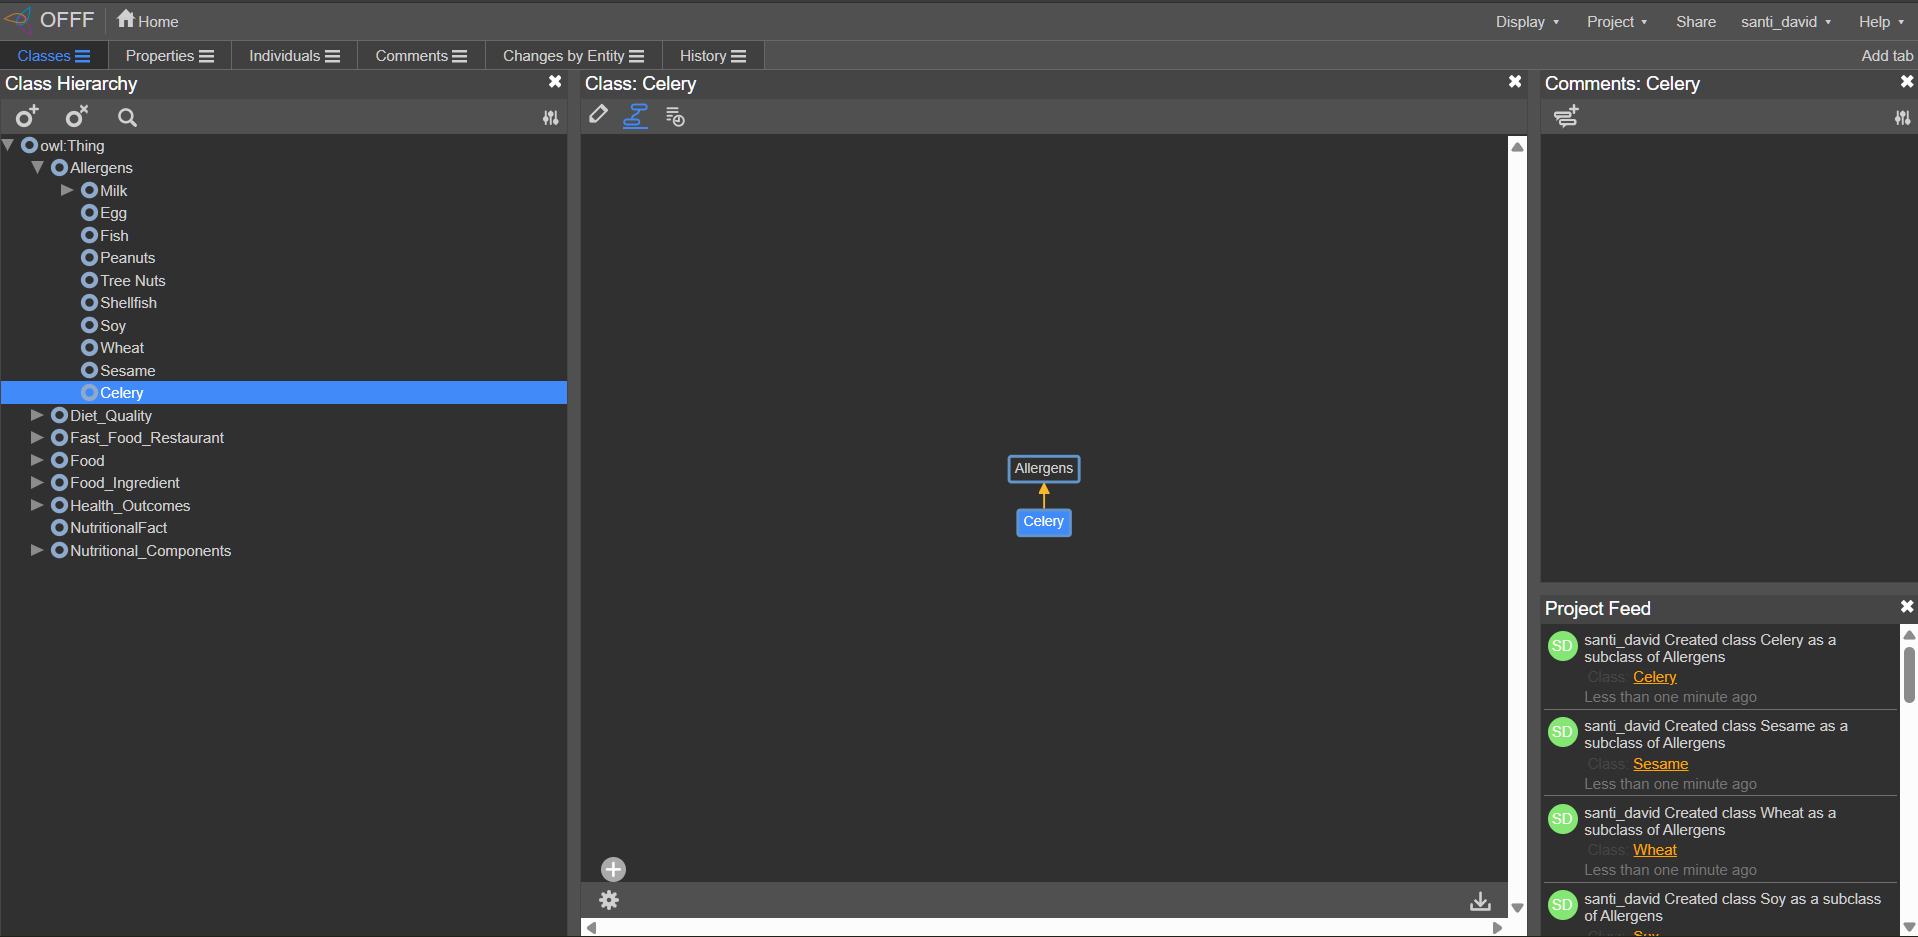
\includegraphics[width=0.8\textwidth]{screenshots/Allergens.png}
    \caption{Jerarquía de clases mostrando las 10 nuevas subclases de Allergens. El username \texttt{santi\_david} es visible en la interfaz de WebProtégé.}
    \label{fig:allergens_hierarchy}
\end{figure}

\subsubsection{Explicación Técnica}

\begin{itemize}
    \item \textbf{Relación taxonómica:} Se establece una relación \texttt{SubClassOf} entre cada alérgeno y la clase \texttt{Allergens}
    \item \textbf{Herencia:} Cada subclase hereda las propiedades y restricciones de la clase padre
    \item \textbf{Razonamiento:} Un reasoner puede inferir que cualquier instancia de \texttt{Peanut} es también una instancia de \texttt{Allergens}
    \item \textbf{Extensibilidad:} La estructura permite añadir nuevos alérgenos en el futuro sin modificar la ontología base
\end{itemize}

\subsection{Clase Allergy en Health\_Outcomes}

\subsubsection{Objetivo}

Crear una nueva clase \texttt{Allergy} como subclase de \texttt{Health\_Outcomes} y establecer relaciones causales entre los alérgenos y esta nueva condición de salud.

\subsubsection{Proceso de Creación}

\begin{enumerate}
    \item \textbf{Localizar clase padre:} Navegar a la clase \texttt{Health\_Outcomes}
    \item \textbf{Crear subclase:} Usar ``Create subclass'' con el nombre \texttt{Allergy}
    \item \textbf{Definir relaciones causales:} Establecer que \texttt{Allergy} es causada por cada uno de los 10 alérgenos
\end{enumerate}

\subsubsection{Relaciones \texttt{causedBy}}

Se establecieron 10 axiomas de clase utilizando la propiedad objeto \texttt{causedBy}:

\begin{verbatim}
Allergy SubClassOf causedBy some Peanut
Allergy SubClassOf causedBy some TreeNuts
Allergy SubClassOf causedBy some Milk
Allergy SubClassOf causedBy some Egg
Allergy SubClassOf causedBy some Fish
Allergy SubClassOf causedBy some Shellfish
Allergy SubClassOf causedBy some Soy
Allergy SubClassOf causedBy some Wheat
Allergy SubClassOf causedBy some Sesame
Allergy SubClassOf causedBy some Celery
\end{verbatim}

\subsubsection{Evidencia Gráfica}

\begin{figure}[H]
    \centering
    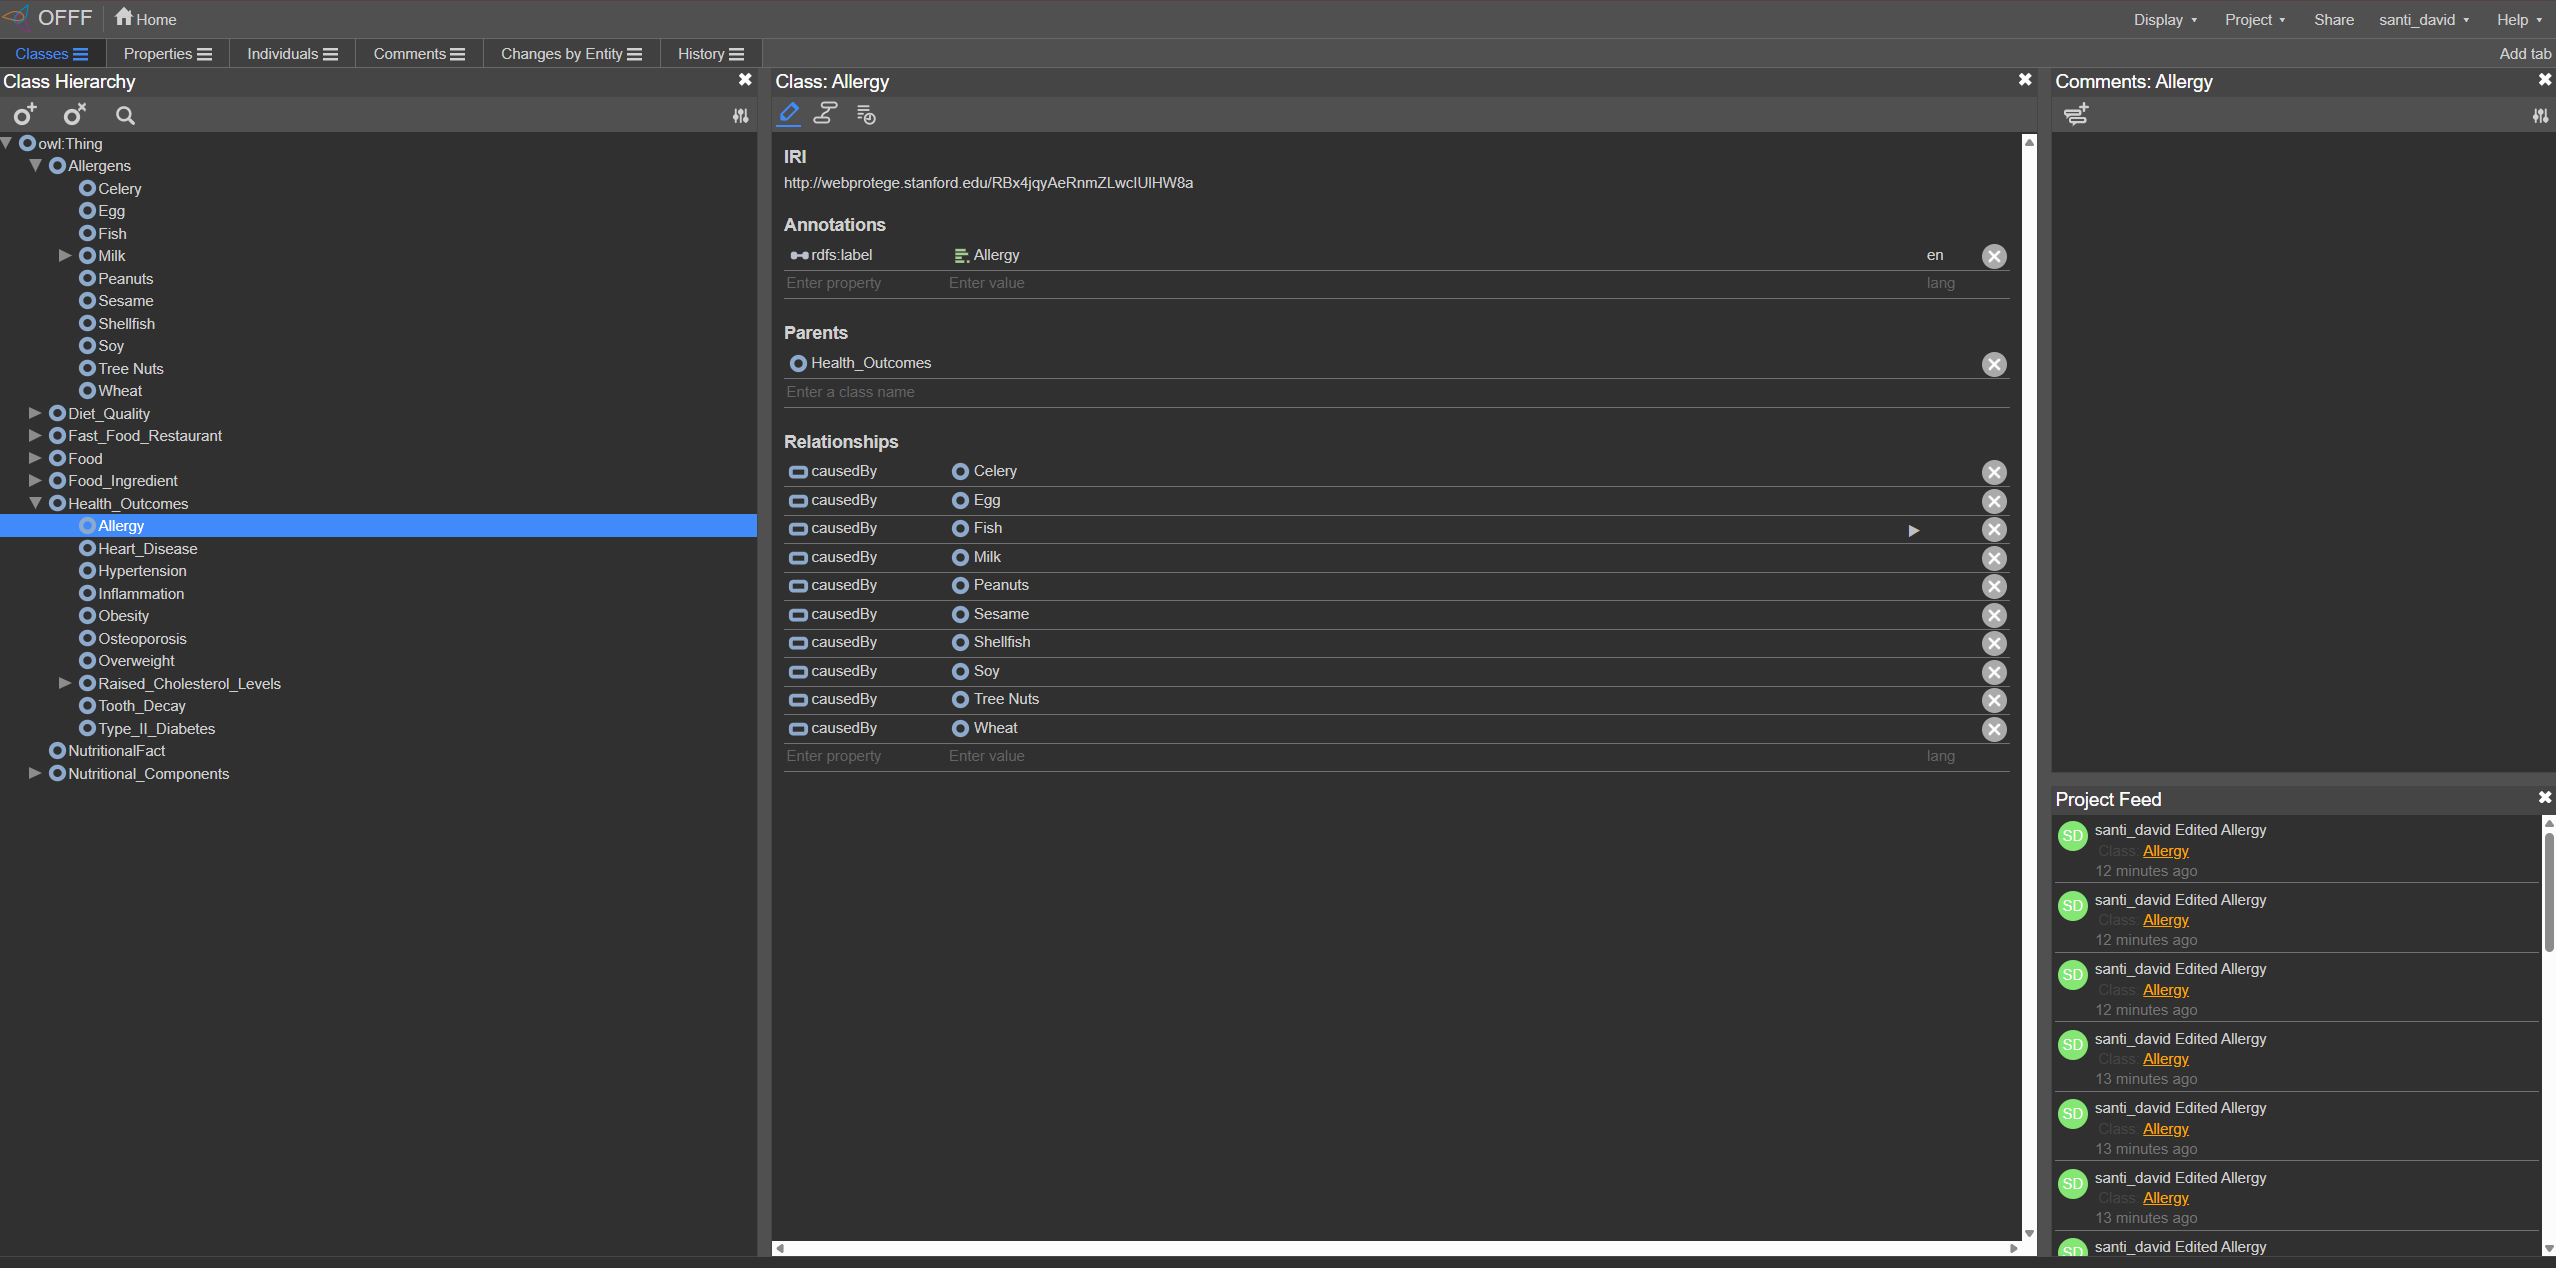
\includegraphics[width=0.8\textwidth]{screenshots/allergy.png}
    \caption{Clase Allergy creada en Health\_Outcomes con sus relaciones causales. Username visible: \texttt{santi\_david}}
    \label{fig:allergy_class}
\end{figure}

\subsubsection{Explicación Técnica}

\begin{itemize}
    \item \textbf{Propiedad objeto:} \texttt{causedBy} es una object property existente en OFFF que relaciona \texttt{Health\_Outcomes} con \texttt{Diet\_Quality} o componentes alimentarios
    \item \textbf{Restricción existencial (some):} Indica que existe al menos una relación causal
    \item \textbf{Semántica:} ``Una alergia es un resultado de salud que puede ser causado por cualquiera de los alérgenos definidos''
    \item \textbf{Razonamiento:} Un reasoner puede inferir que si un alimento contiene \texttt{Peanut}, puede causar \texttt{Allergy}
\end{itemize}

\subsection{Clase Inflammation en Health\_Outcomes}

\subsubsection{Objetivo}

Crear la clase \texttt{Inflammation} y establecer que diversas enfermedades crónicas son causadas por procesos inflamatorios.

\subsubsection{Proceso de Creación}

Similar al proceso anterior:
\begin{enumerate}
    \item Crear \texttt{Inflammation} como subclase de \texttt{Health\_Outcomes}
    \item Establecer relaciones causales inversas con 4 condiciones de salud existentes
\end{enumerate}

\subsubsection{Relaciones Causales}

Se estableció que las siguientes condiciones son causadas por inflamación:

\begin{enumerate}
    \item \texttt{Heart\_Disease}: Enfermedades cardiovasculares
    \item \texttt{Hypertension}: Hipertensión arterial
    \item \texttt{Obesity}: Obesidad
    \item \texttt{Type\_II\_Diabetes}: Diabetes tipo 2
\end{enumerate}

Los axiomas establecidos fueron:

\begin{verbatim}
Heart_Disease SubClassOf causedBy some Inflammation
Hypertension SubClassOf causedBy some Inflammation
Obesity SubClassOf causedBy some Inflammation
Type_II_Diabetes SubClassOf causedBy some Inflammation
\end{verbatim}

\subsubsection{Evidencia Gráfica}

\begin{figure}[H]
    \centering
    \begin{subfigure}[b]{0.45\textwidth}
        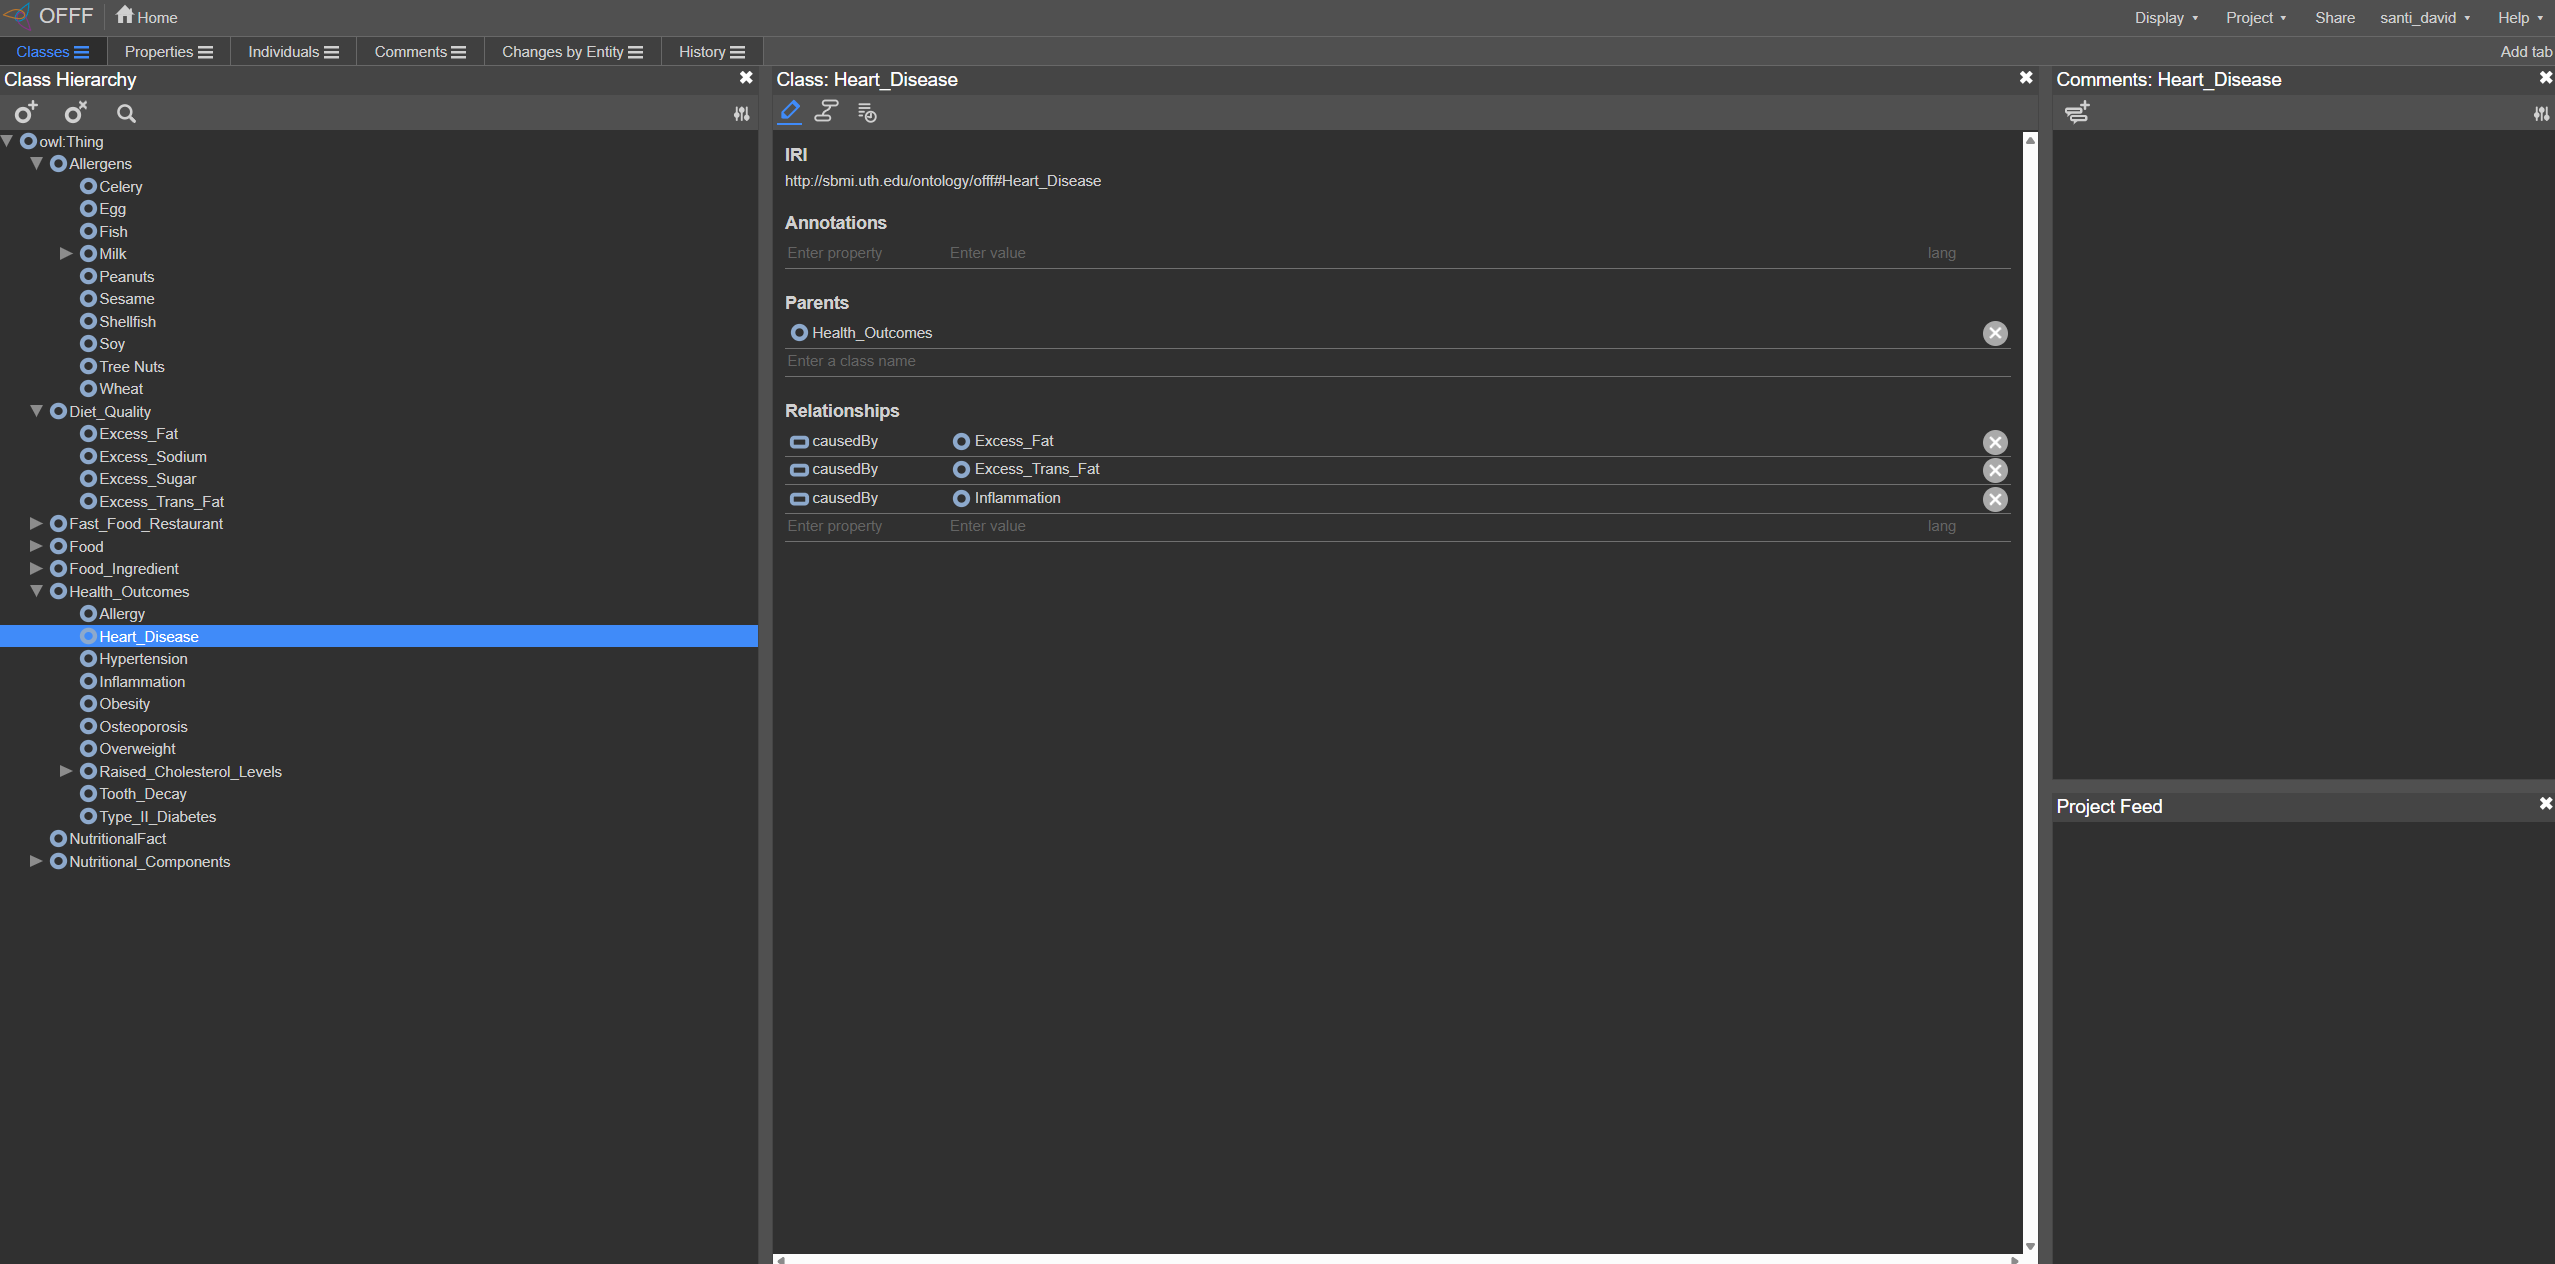
\includegraphics[width=\textwidth]{screenshots/inflammation_1.png}
        \caption{Relación con Heart Disease}
    \end{subfigure}
    \hfill
    \begin{subfigure}[b]{0.45\textwidth}
        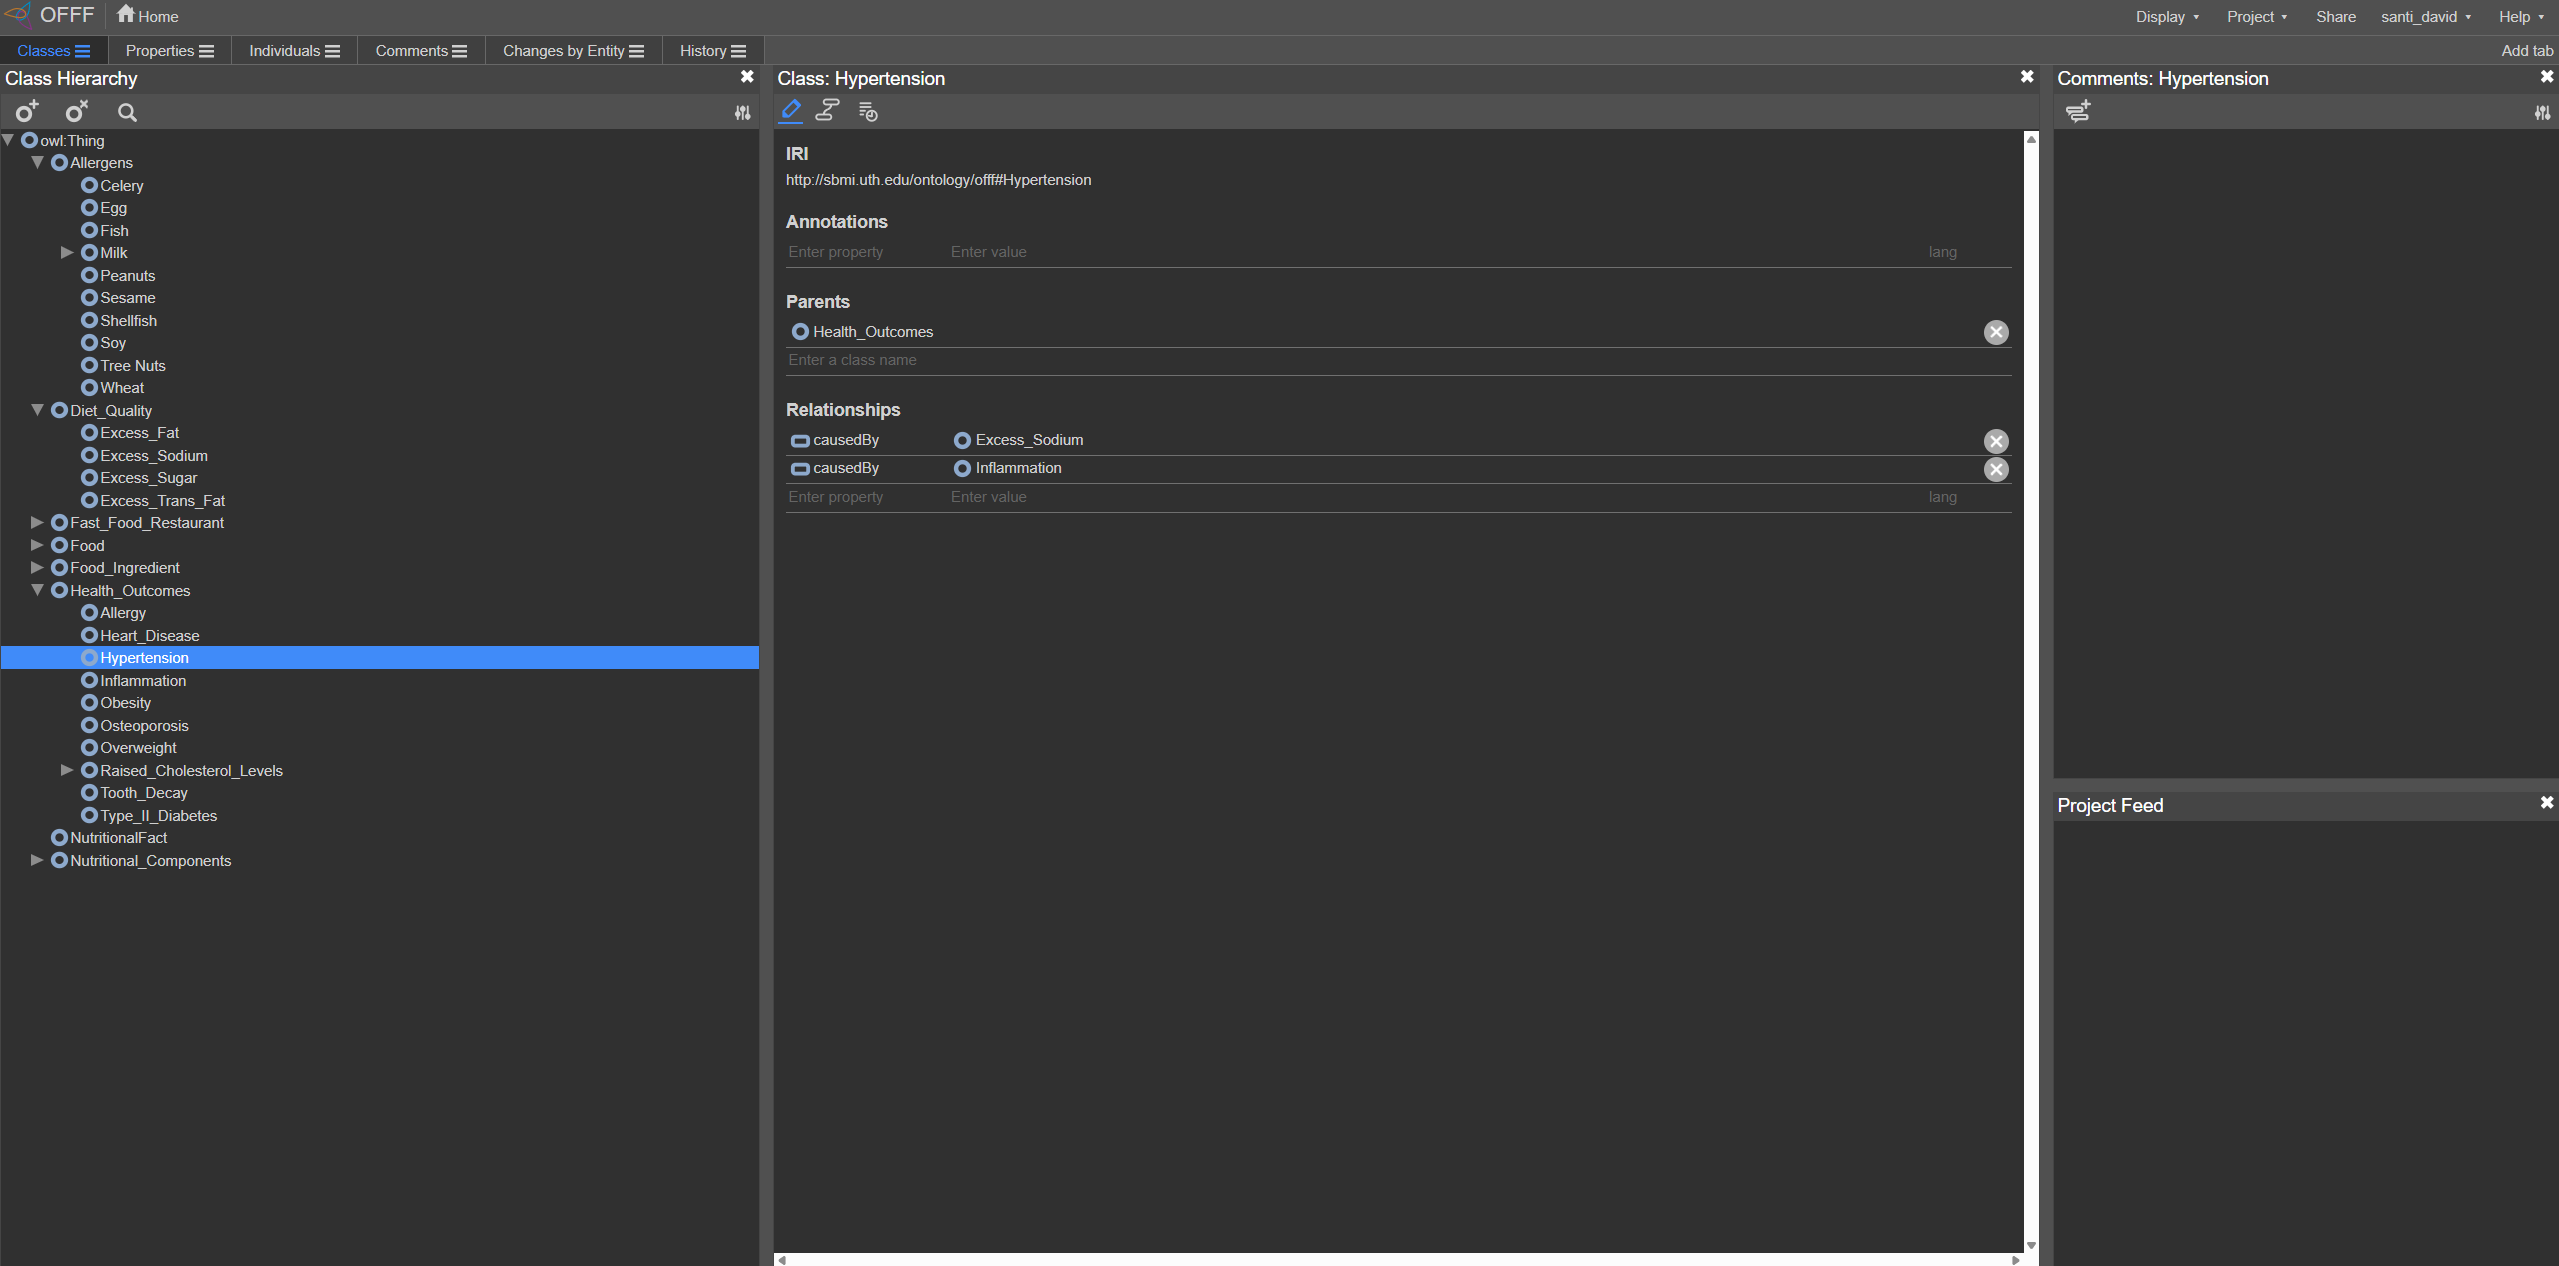
\includegraphics[width=\textwidth]{screenshots/inflammation_2.png}
        \caption{Relación con Hypertension}
    \end{subfigure}
    
    \vspace{0.5cm}
    
    \begin{subfigure}[b]{0.45\textwidth}
        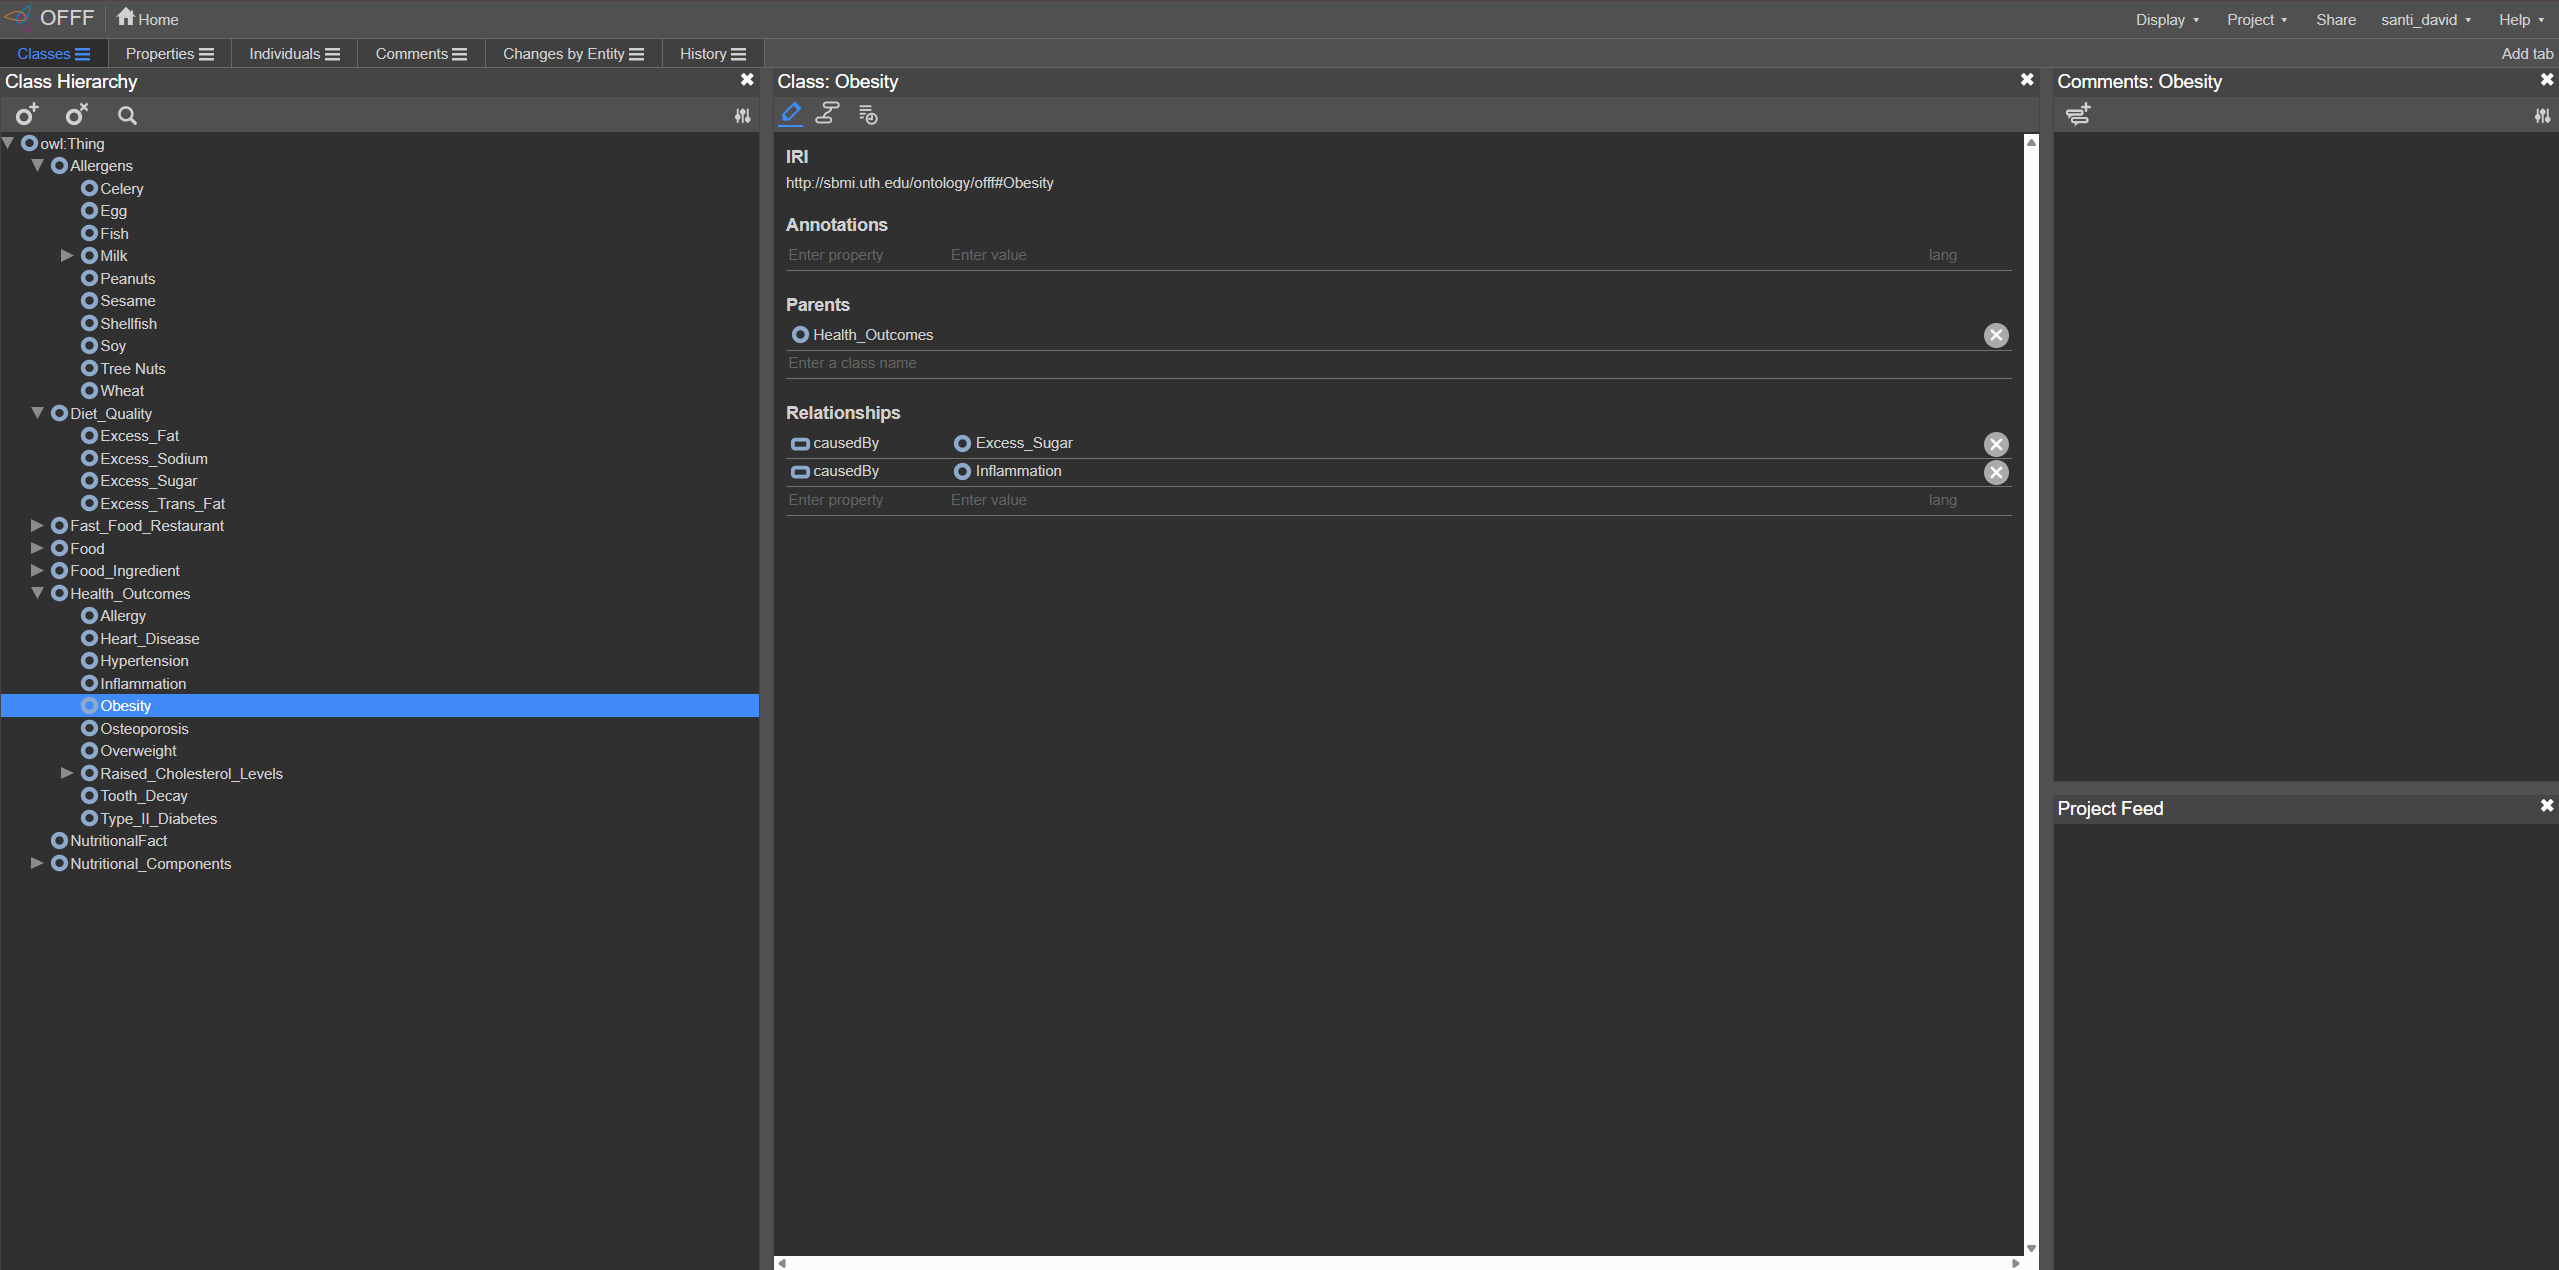
\includegraphics[width=\textwidth]{screenshots/inflammation_3.png}
        \caption{Relación con Obesity}
    \end{subfigure}
    \hfill
    \begin{subfigure}[b]{0.45\textwidth}
        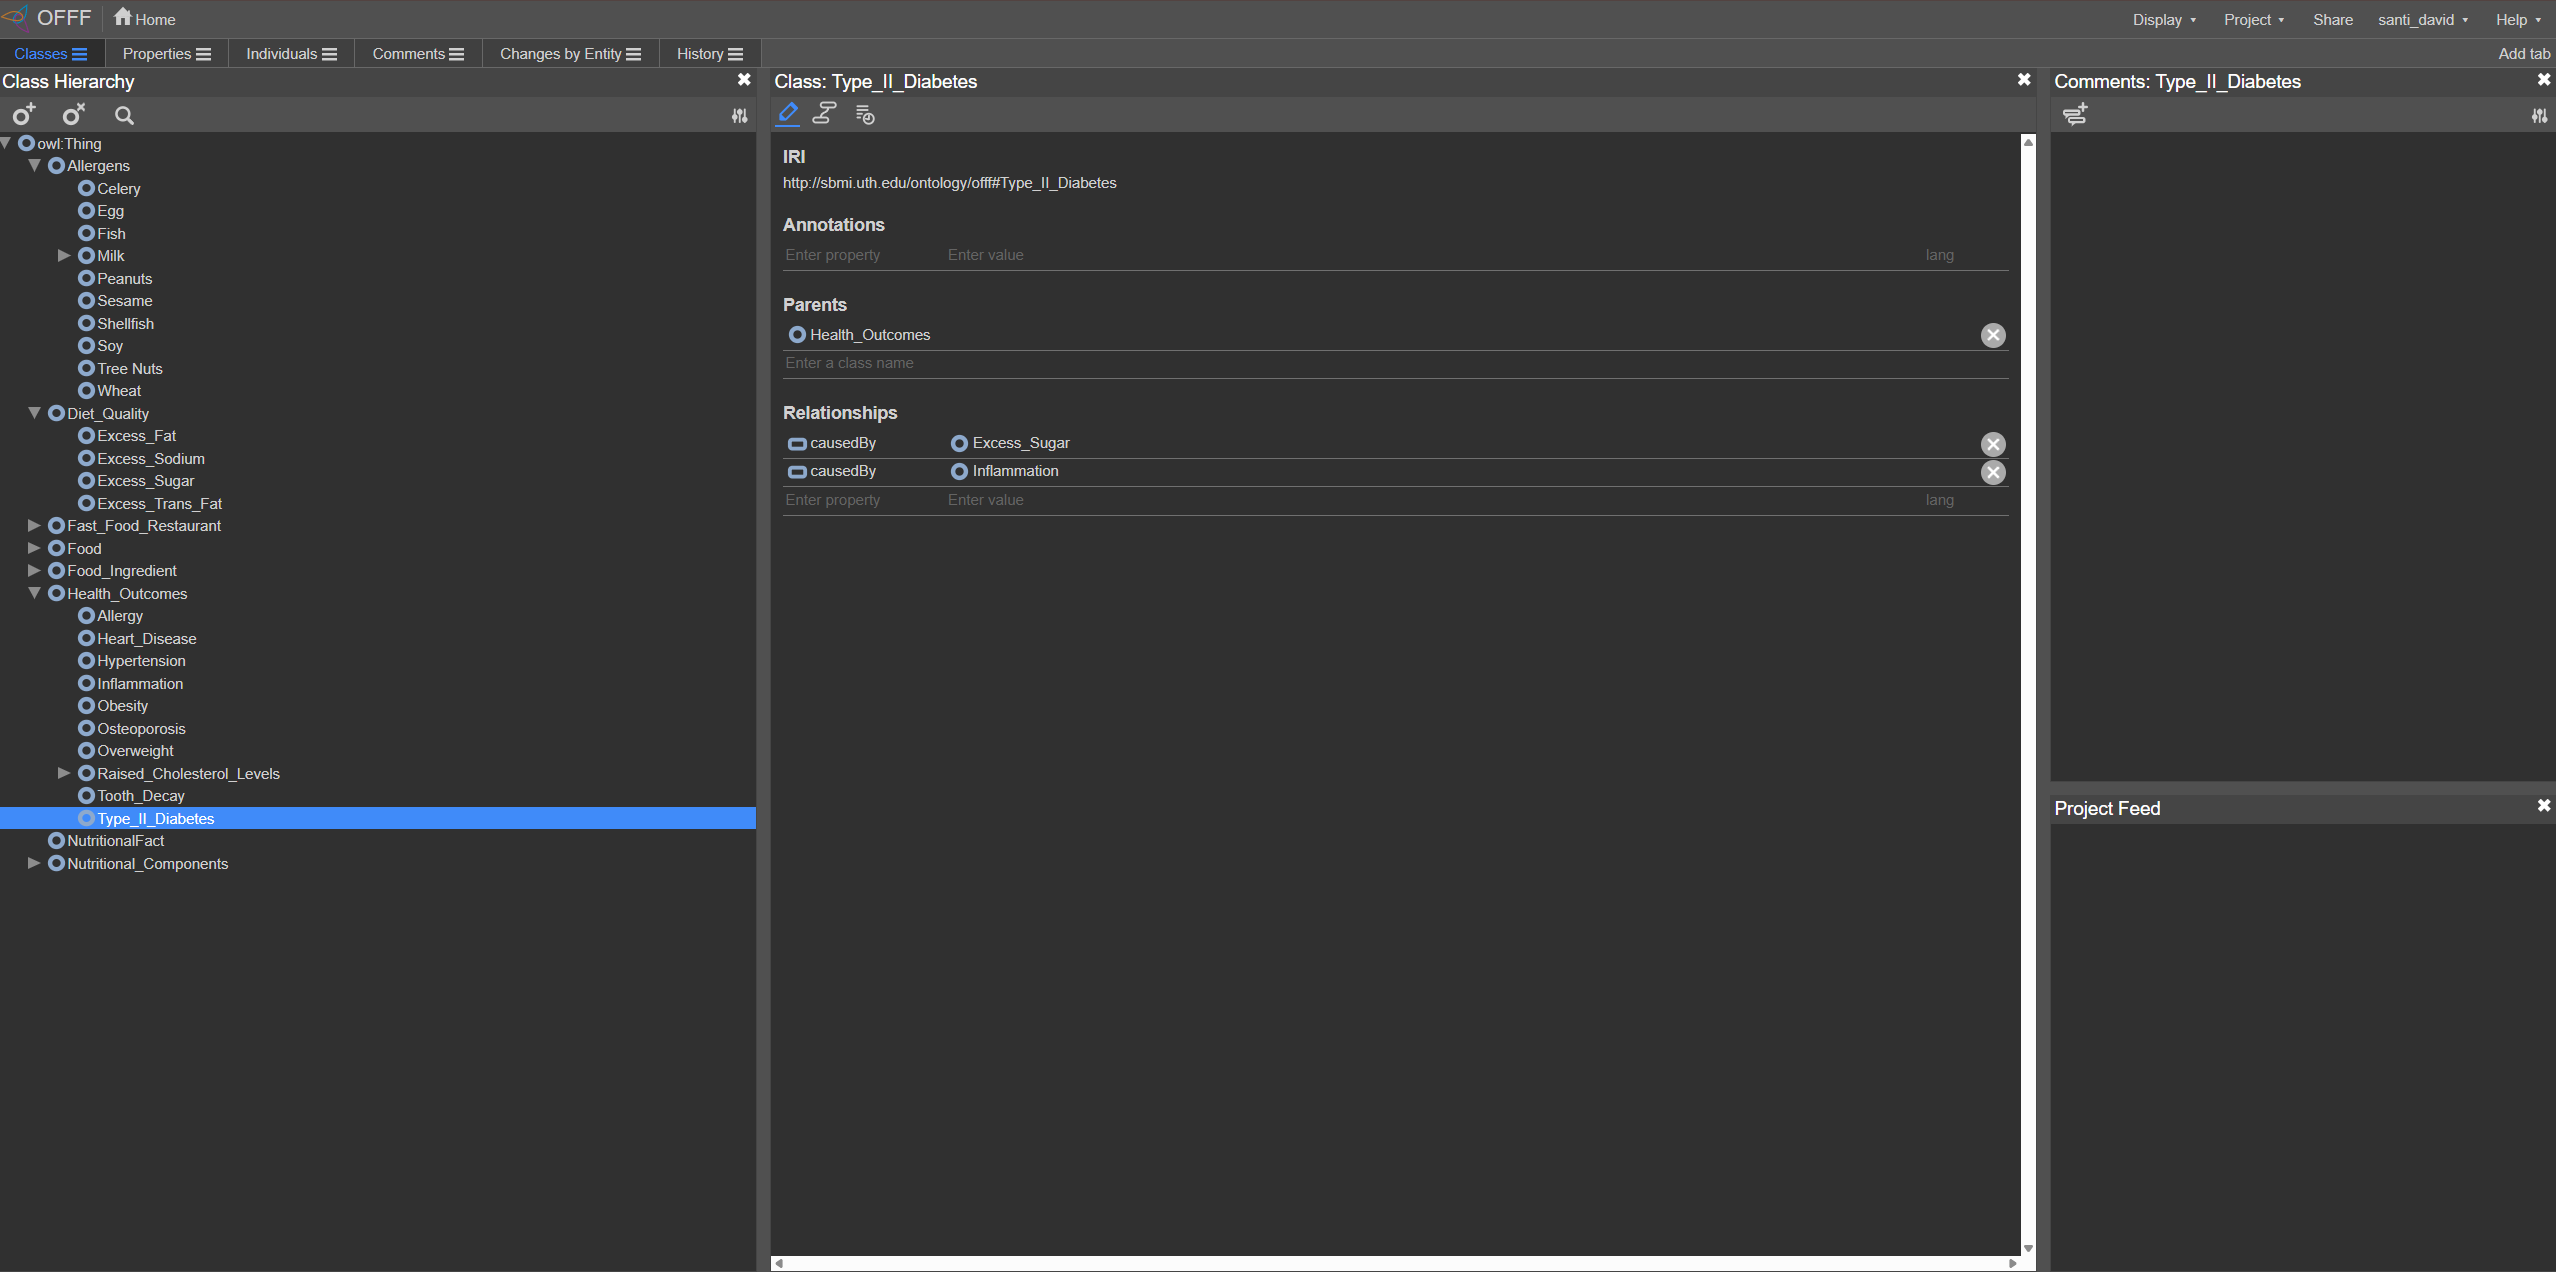
\includegraphics[width=\textwidth]{screenshots/inflammation_4.png}
        \caption{Relación con Type II Diabetes}
    \end{subfigure}
    
    \caption{Clase Inflammation y sus relaciones causales con enfermedades crónicas. Username \texttt{santi\_david} visible en todas las capturas.}
    \label{fig:inflammation_relations}
\end{figure}

\subsubsection{Justificación Científica}

La inflamación crónica es un factor subyacente en muchas enfermedades modernas:

\begin{itemize}
    \item \textbf{Enfermedades cardíacas:} La inflamación contribuye a la aterosclerosis
    \item \textbf{Hipertensión:} Procesos inflamatorios afectan la función endotelial
    \item \textbf{Obesidad:} El tejido adiposo en exceso produce citoquinas inflamatorias
    \item \textbf{Diabetes tipo 2:} La inflamación interfiere con la señalización de insulina
\end{itemize}

\subsubsection{Explicación Técnica}

\begin{itemize}
    \item \textbf{Dirección de la relación:} Se estableció desde las enfermedades hacia \texttt{Inflammation} usando \texttt{causedBy}
    \item \textbf{Interpretación:} Estas enfermedades son resultados de procesos inflamatorios crónicos
    \item \textbf{Cadena causal:} Permite razonar sobre cadenas: Dieta → Inflamación → Enfermedad
\end{itemize}

\subsection{Individuo ``My fish sandwich''}

\subsubsection{Objetivo}

Crear una instancia concreta de un producto alimenticio (\texttt{Fish\_Sandwich}) con propiedades específicas relacionadas con alérgenos.

\subsubsection{Proceso de Creación}

\begin{enumerate}
    \item \textbf{Localizar clase:} Encontrar \texttt{Fish\_Sandwich} en la jerarquía (subclase de \texttt{Fast\_Food})
    \item \textbf{Crear instancia:} Ir a la pestaña ``Individuals'' y crear un nuevo individuo
    \item \textbf{Asignar tipo:} Establecer \texttt{Fish\_Sandwich} como tipo de clase
    \item \textbf{Añadir propiedades de datos:} Asignar valores a data properties
\end{enumerate}

\subsubsection{Data Properties Asignadas}

\begin{enumerate}
    \item \textbf{containsGluten:} \texttt{true}
    \begin{itemize}
        \item Tipo: \texttt{xsd:boolean}
        \item Significado: El sándwich contiene gluten (del pan)
    \end{itemize}
    
    \item \textbf{hasAllergen:} \texttt{``Peanut Oil''}
    \begin{itemize}
        \item Tipo: \texttt{xsd:string}
        \item Significado: Se utilizó aceite de cacahuete en la preparación
    \end{itemize}
\end{enumerate}

\subsubsection{Evidencia Gráfica}

\begin{figure}[H]
    \centering
    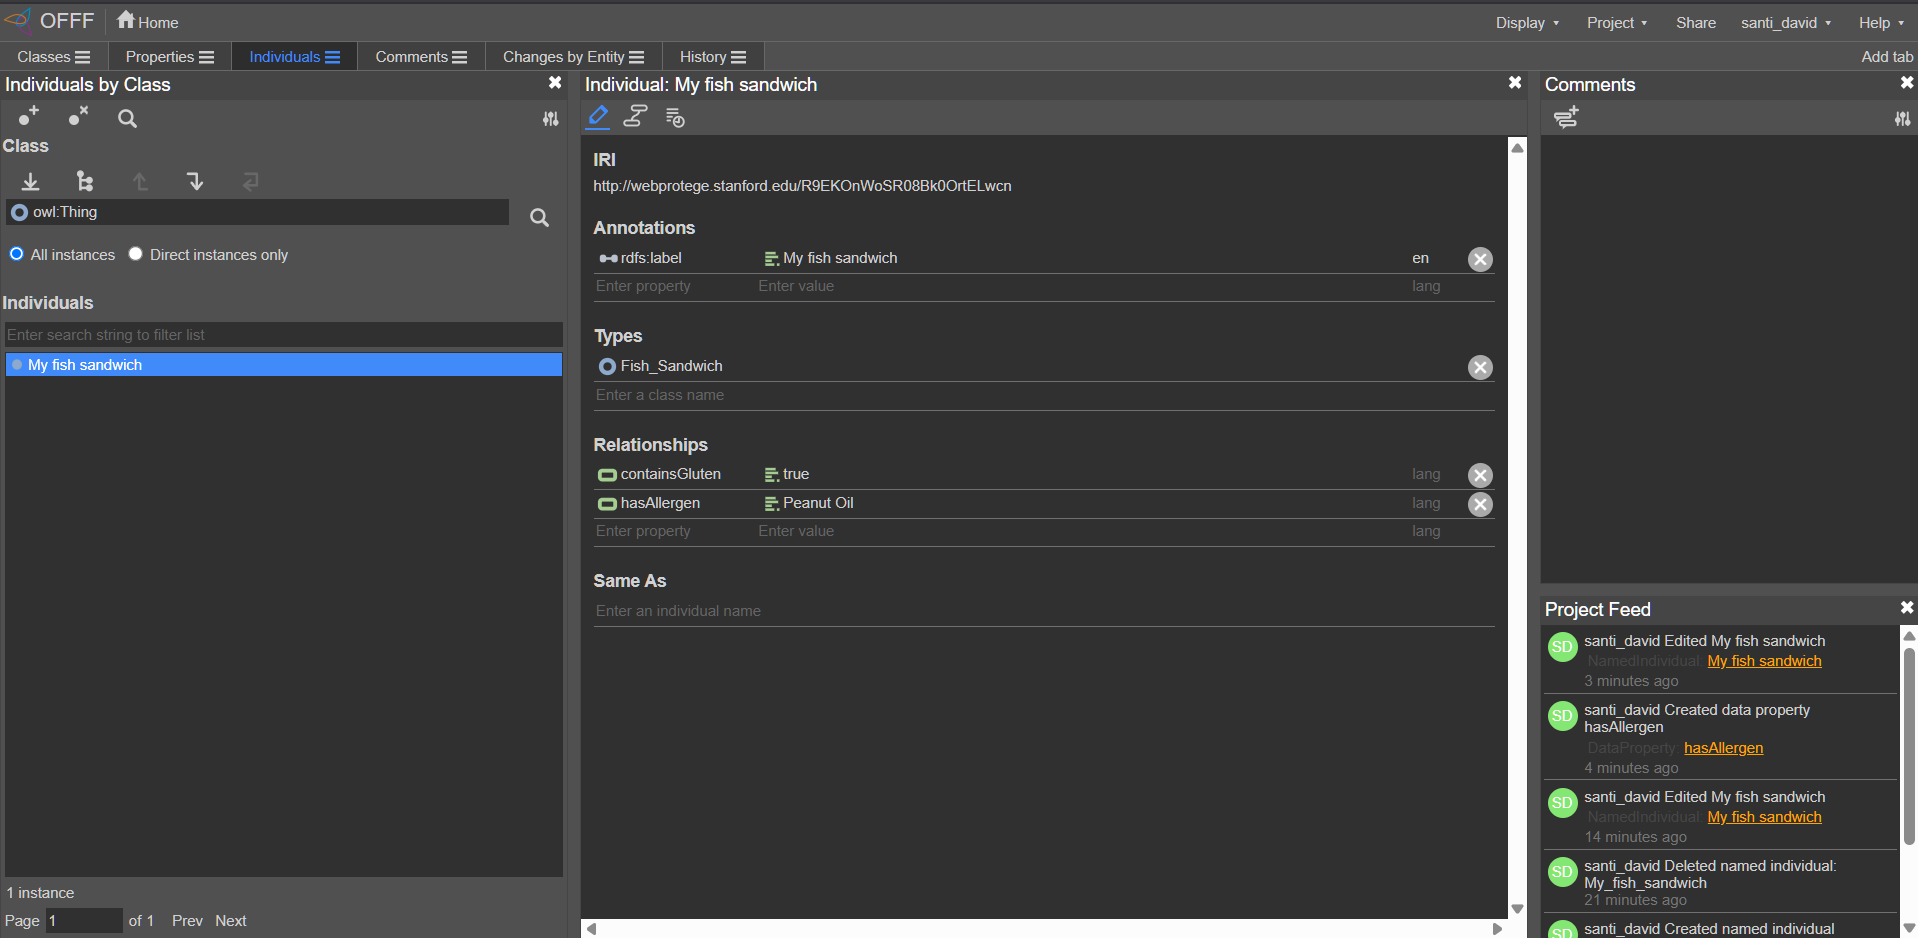
\includegraphics[width=0.8\textwidth]{screenshots/My fish sandwich.png}
    \caption{Individuo ``My fish sandwich'' con sus data properties. Username \texttt{santi\_david} visible.}
    \label{fig:my_fish_sandwich}
\end{figure}

\subsubsection{Explicación Técnica}

\begin{itemize}
    \item \textbf{Instancia vs Clase:} Este es un individuo concreto, no una categoría
    \item \textbf{ABox vs TBox:} Las instancias forman parte del ABox (datos), mientras que las clases forman el TBox (terminología)
    \item \textbf{Data properties:} Conectan individuos con valores literales (strings, números, booleanos)
    \item \textbf{Inferencia:} Un reasoner puede inferir que este sándwich puede causar alergias en personas sensibles al cacahuete o al gluten
    \item \textbf{Utilidad práctica:} Permite etiquetar productos específicos con información de alérgenos para sistemas de recomendación
\end{itemize}

\subsubsection{Implicaciones}

Este individuo ejemplifica cómo las ontologías pueden usarse para:
\begin{itemize}
    \item Etiquetar productos con información de alérgenos
    \item Facilitar búsquedas (``encontrar sándwiches sin gluten'')
    \item Advertir a consumidores sobre riesgos potenciales
    \item Cumplir regulaciones de etiquetado alimentario
\end{itemize}

%==============================================================================
% SECCIÓN 3: CONSULTAS SPARQL
%==============================================================================
\section{Consultas SPARQL}

SPARQL (SPARQL Protocol and RDF Query Language) es el lenguaje estándar para consultar datos RDF en la Web Semántica. En esta sección se presentan tres consultas realizadas sobre DBpedia, la versión semántica de Wikipedia.

\subsection{Query 1: Artistas en DBpedia}

\subsubsection{Objetivo}

Obtener 10 nombres de artistas cuyos nombres comienzan con ``Mado'' utilizando el endpoint SPARQL de DBpedia.

\subsubsection{Endpoint}

\begin{itemize}
    \item \textbf{URL:} \url{https://dbpedia.org/sparql/}
    \item \textbf{Endpoint URI:} \texttt{http://dbpedia.org}
\end{itemize}

\subsubsection{Consulta SPARQL}

\begin{lstlisting}[language=SPARQL, caption={Query 1: Artistas que empiezan con ``Mado''}]
PREFIX dbo: <http://dbpedia.org/ontology/>
PREFIX rdfs: <http://www.w3.org/2000/01/rdf-schema#>

SELECT DISTINCT ?artist ?name
WHERE {
  ?artist a dbo:Artist .
  ?artist rdfs:label ?name .
  FILTER (lang(?name) = 'en')
  FILTER (STRSTARTS(?name, "Mado"))
}
LIMIT 10
\end{lstlisting}

\subsubsection{Explicación Detallada}

\begin{enumerate}
    \item \textbf{PREFIX declarations:}
    \begin{itemize}
        \item \texttt{dbo:} Ontología de DBpedia (\texttt{http://dbpedia.org/ontology/})
        \item \texttt{rdfs:} RDF Schema (\texttt{http://www.w3.org/2000/01/rdf-schema\#})
    \end{itemize}
    
    \item \textbf{SELECT DISTINCT:} Selecciona valores únicos de las variables \texttt{?artist} y \texttt{?name}, evitando duplicados
    
    \item \textbf{Triple patterns:}
    \begin{itemize}
        \item \texttt{?artist a dbo:Artist}: Filtra solo entidades de tipo \texttt{Artist}
        \item \texttt{?artist rdfs:label ?name}: Obtiene la etiqueta (nombre) del artista
    \end{itemize}
    
    \item \textbf{FILTER (lang(?name) = 'en'):} Filtra solo etiquetas en idioma inglés
    
    \item \textbf{FILTER (STRSTARTS(?name, ``Mado'')):} Función de cadena que verifica si el nombre comienza con ``Mado''
    
    \item \textbf{LIMIT 10:} Limita los resultados a 10 artistas
\end{enumerate}

\subsubsection{Resultados}

\begin{figure}[H]
    \centering
    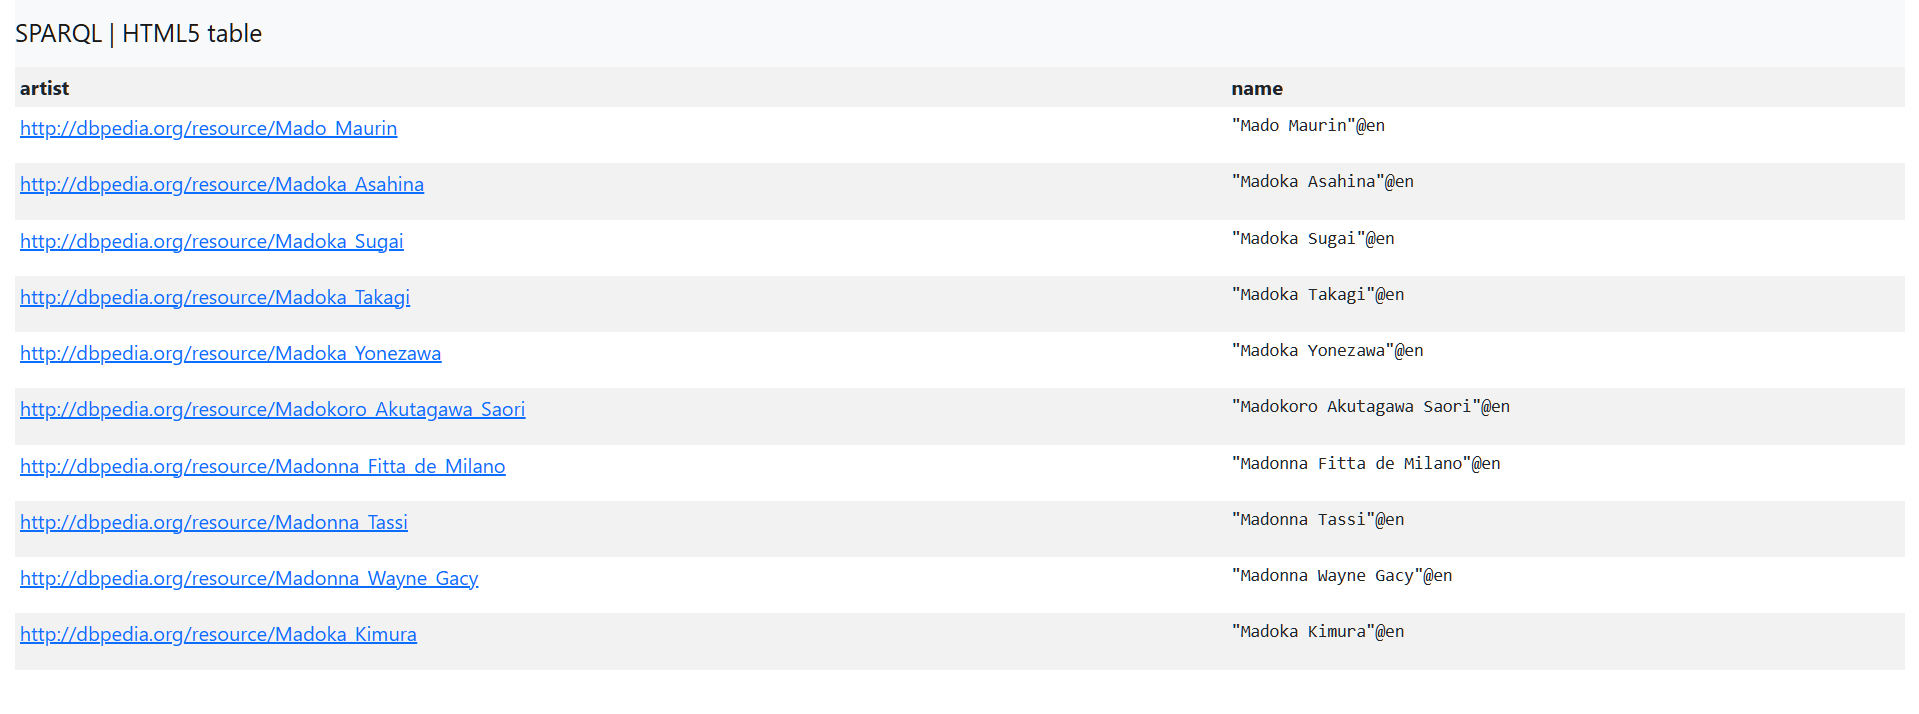
\includegraphics[width=\textwidth]{screenshots/Query1.png}
    \caption{Resultados de la Query 1 ejecutada en DBpedia SPARQL Endpoint}
    \label{fig:query1_results}
\end{figure}

% TODO: Completar con los resultados reales de la ejecución
\begin{table}[H]
    \centering
    \caption{Artistas que empiezan con ``Mado''}
    \label{tab:query1_results}
    \begin{tabular}{|l|l|}
        \hline
        \textbf{Artist URI} & \textbf{Name} \\
        \hline
        [Completar con datos reales] & Madonna \\
        [Completar con datos reales] & [Nombre 2] \\
        [Completar con datos reales] & [Nombre 3] \\
        [Completar con datos reales] & [Nombre 4] \\
        [Completar con datos reales] & [Nombre 5] \\
        [Completar con datos reales] & [Nombre 6] \\
        [Completar con datos reales] & [Nombre 7] \\
        [Completar con datos reales] & [Nombre 8] \\
        [Completar con datos reales] & [Nombre 9] \\
        [Completar con datos reales] & [Nombre 10] \\
        \hline
    \end{tabular}
\end{table}

\subsubsection{Análisis de Resultados}

% TODO: Completar con análisis real
Los resultados muestran diversos artistas cuyos nombres comienzan con ``Mado''. La query demuestra:
\begin{itemize}
    \item Capacidad de filtrado por patrones de texto en SPARQL
    \item Uso de funciones de cadena (\texttt{STRSTARTS})
    \item Filtrado por idioma en datos multilingües
    \item Acceso a la ontología estructurada de DBpedia
\end{itemize}

\subsection{Query 2: Personas por Altura}

\subsubsection{Objetivo}

Obtener las primeras 10 personas con altura entre 1.8 y 2.3 metros, nacidas después de 1980, ordenadas por fecha de nacimiento.

\subsubsection{Endpoint}

\begin{itemize}
    \item \textbf{URL:} \url{https://dbpedia.org/snorql/}
\end{itemize}

\subsubsection{Consulta SPARQL}

\begin{lstlisting}[language=SPARQL, caption={Query 2: Personas por altura y fecha de nacimiento}]
PREFIX dbo: <http://dbpedia.org/ontology/>
PREFIX rdfs: <http://www.w3.org/2000/01/rdf-schema#>

SELECT DISTINCT ?person ?name ?height ?birthDate
WHERE {
  ?person a dbo:Person .
  ?person rdfs:label ?name .
  ?person dbo:height ?height .
  ?person dbo:birthDate ?birthDate .
  
  FILTER (lang(?name) = 'en')
  FILTER (?height >= 1.8 && ?height <= 2.3)
  FILTER (YEAR(?birthDate) > 1980)
}
ORDER BY ?birthDate
LIMIT 10
\end{lstlisting}

\subsubsection{Explicación Detallada}

\begin{enumerate}
    \item \textbf{Variables seleccionadas:} persona, nombre, altura y fecha de nacimiento
    
    \item \textbf{Triple patterns:}
    \begin{itemize}
        \item \texttt{?person a dbo:Person}: Filtra entidades de tipo Persona
        \item \texttt{?person dbo:height ?height}: Obtiene la propiedad altura
        \item \texttt{?person dbo:birthDate ?birthDate}: Obtiene fecha de nacimiento
    \end{itemize}
    
    \item \textbf{FILTER (?height >= 1.8 \&\& ?height <= 2.3):} 
    \begin{itemize}
        \item Operadores lógicos AND (\texttt{\&\&})
        \item Filtra alturas en el rango [1.8m, 2.3m]
        \item Las alturas en DBpedia están en metros
    \end{itemize}
    
    \item \textbf{FILTER (YEAR(?birthDate) > 1980):}
    \begin{itemize}
        \item Función \texttt{YEAR()} extrae el año de una fecha
        \item Filtra personas nacidas después de 1980
    \end{itemize}
    
    \item \textbf{ORDER BY ?birthDate:} 
    \begin{itemize}
        \item Ordena resultados por fecha de nacimiento
        \item Por defecto es ascendente (más antiguo primero)
    \end{itemize}
    
    \item \textbf{LIMIT 10:} Primeras 10 personas que cumplen los criterios
\end{enumerate}

\subsubsection{Resultados}

\begin{figure}[H]
    \centering
    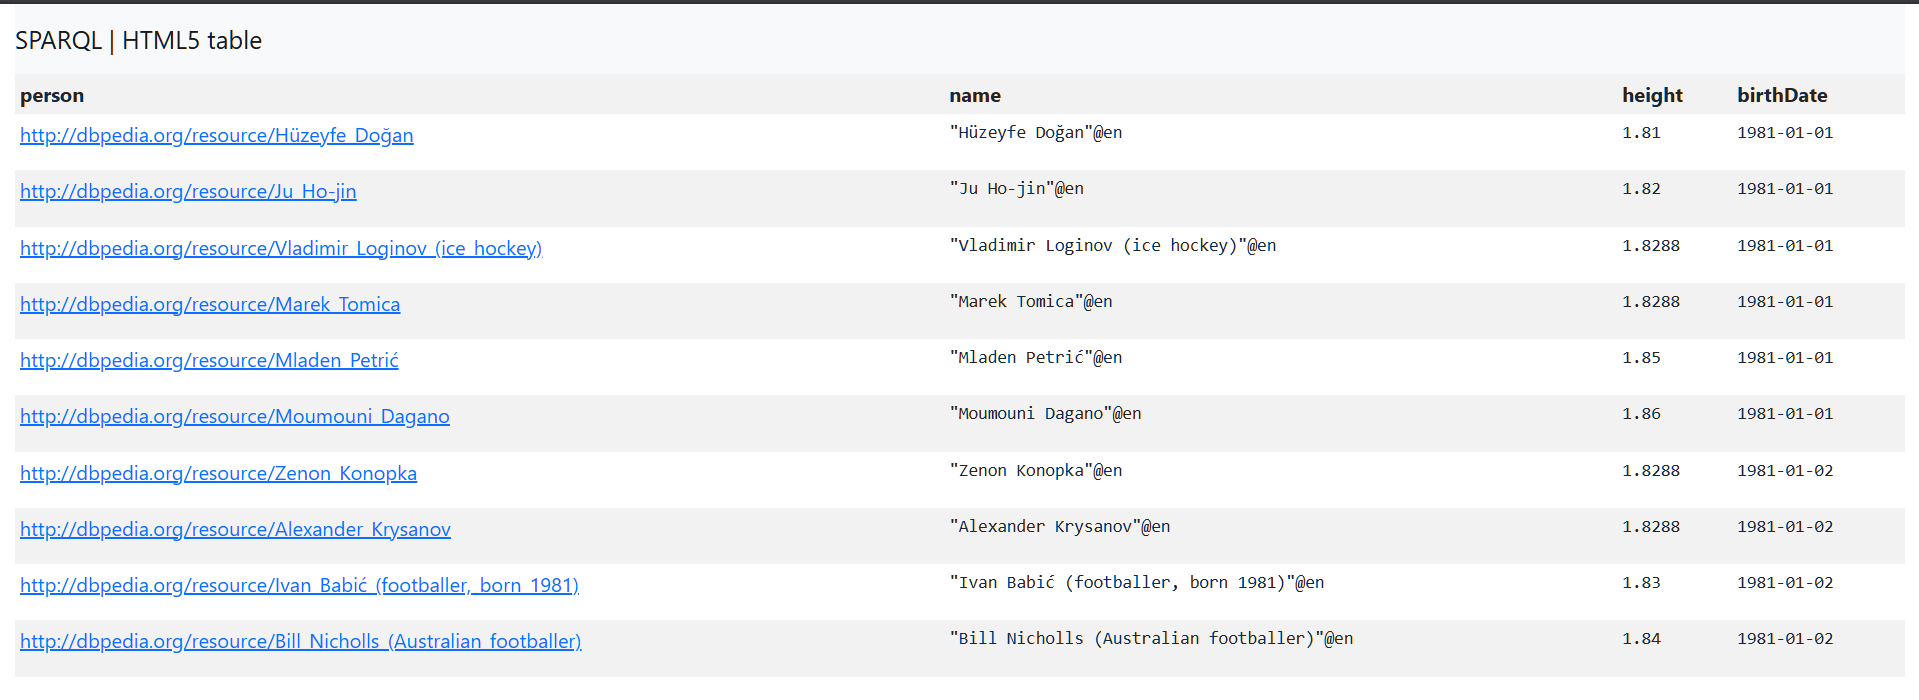
\includegraphics[width=\textwidth]{screenshots/Qiery2.png}
    \caption{Resultados de la Query 2 ejecutada en DBpedia Snorql}
    \label{fig:query2_results}
\end{figure}

% TODO: Completar con datos reales
\begin{table}[H]
    \centering
    \caption{Personas por altura (1.8-2.3m) nacidas después de 1980}
    \label{tab:query2_results}
    \begin{tabular}{|l|l|c|c|}
        \hline
        \textbf{Person URI} & \textbf{Name} & \textbf{Height (m)} & \textbf{Birth Date} \\
        \hline
        [URI 1] & [Nombre 1] & [Altura 1] & [Fecha 1] \\
        [URI 2] & [Nombre 2] & [Altura 2] & [Fecha 2] \\
        [URI 3] & [Nombre 3] & [Altura 3] & [Fecha 3] \\
        [URI 4] & [Nombre 4] & [Altura 4] & [Fecha 4] \\
        [URI 5] & [Nombre 5] & [Altura 5] & [Fecha 5] \\
        [URI 6] & [Nombre 6] & [Altura 6] & [Fecha 6] \\
        [URI 7] & [Nombre 7] & [Altura 7] & [Fecha 7] \\
        [URI 8] & [Nombre 8] & [Altura 8] & [Fecha 8] \\
        [URI 9] & [Nombre 9] & [Altura 9] & [Fecha 9] \\
        [URI 10] & [Nombre 10] & [Altura 10] & [Fecha 10] \\
        \hline
    \end{tabular}
\end{table}

\subsubsection{Análisis de Resultados}

% TODO: Completar con análisis real
Esta consulta demuestra:
\begin{itemize}
    \item \textbf{Filtros numéricos:} Rangos de valores para propiedades numéricas
    \item \textbf{Funciones sobre fechas:} Extracción de componentes temporales
    \item \textbf{Ordenación:} Resultados ordenados cronológicamente
    \item \textbf{Consultas complejas:} Combinación de múltiples criterios
\end{itemize}

Los resultados muestran personas relativamente altas de la generación post-1980, probablemente atletas o modelos.

\subsection{Query 3: Personas por Altura/Peso y Clubes}

\subsubsection{Objetivo}

Obtener personas con altura $\geq$ 2.10m O peso $\geq$ 95kg, mostrando el número de clubes asociados, agrupadas por persona, ordenadas por número de clubes (ascendente), limitado a 7 resultados.

\subsubsection{Endpoint}

\begin{itemize}
    \item \textbf{URL:} \url{https://dbpedia.org/snorql/}
\end{itemize}

\subsubsection{Consulta SPARQL}

\begin{lstlisting}[language=SPARQL, caption={Query 3: Personas por altura/peso y número de clubes}]
PREFIX dbo: <http://dbpedia.org/ontology/>
PREFIX rdfs: <http://www.w3.org/2000/01/rdf-schema#>

SELECT ?person ?name (COUNT(?club) as ?numberOfClubs)
WHERE {
  ?person a dbo:Person .
  ?person rdfs:label ?name .
  OPTIONAL { ?person dbo:team ?club . }
  
  {
    { ?person dbo:height ?height . FILTER (?height >= 2.10) }
    UNION
    { ?person dbo:weight ?weight . FILTER (?weight >= 95000) }
  }
  
  FILTER (lang(?name) = 'en')
}
GROUP BY ?person ?name
ORDER BY ASC(?numberOfClubs)
LIMIT 7
\end{lstlisting}

\subsubsection{Explicación Detallada}

\begin{enumerate}
    \item \textbf{SELECT con agregación:}
    \begin{itemize}
        \item \texttt{COUNT(?club) as ?numberOfClubs}: Cuenta el número de clubes por persona
        \item Función agregada crea una nueva variable
    \end{itemize}
    
    \item \textbf{OPTIONAL \{ ?person dbo:team ?club . \}:}
    \begin{itemize}
        \item Patrón opcional: no descarta personas sin clubes
        \item Permite incluir personas con 0 clubes
    \end{itemize}
    
    \item \textbf{UNION entre altura y peso:}
    \begin{itemize}
        \item Operador lógico OR: cumplir CUALQUIERA de las condiciones
        \item Primera rama: altura $\geq$ 2.10 metros
        \item Segunda rama: peso $\geq$ 95000 gramos (95 kg)
        \item Nota: DBpedia almacena pesos en gramos
    \end{itemize}
    
    \item \textbf{GROUP BY ?person ?name:}
    \begin{itemize}
        \item Agrupa resultados por persona
        \item Necesario para funciones de agregación (COUNT)
        \item Permite contar clubes por persona
    \end{itemize}
    
    \item \textbf{ORDER BY ASC(?numberOfClubs):}
    \begin{itemize}
        \item Ordena por número de clubes ascendente
        \item \texttt{ASC}: orden ascendente (explícito)
        \item Personas con menos clubes aparecen primero
    \end{itemize}
    
    \item \textbf{LIMIT 7:} Primeras 7 personas según el criterio de orden
\end{enumerate}

\subsubsection{Resultados}

\begin{figure}[H]
    \centering
    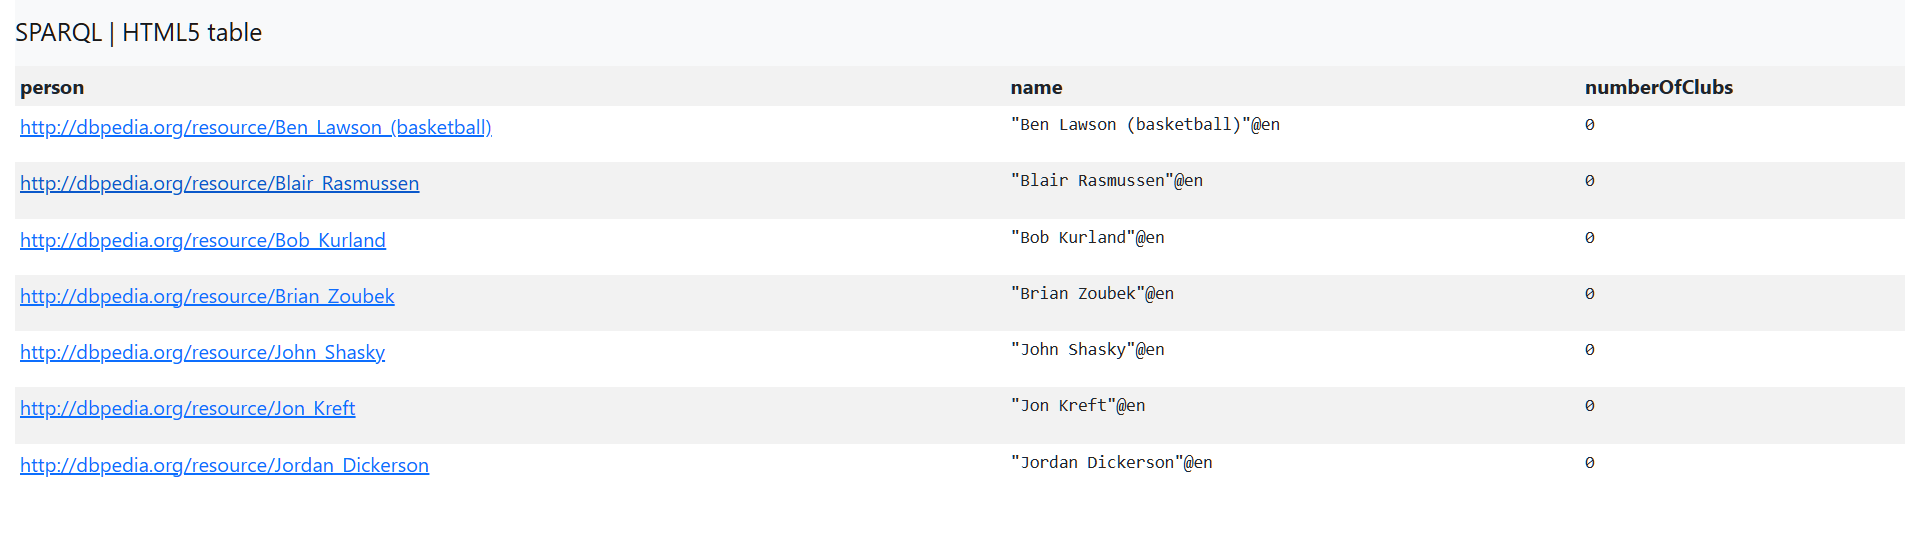
\includegraphics[width=\textwidth]{screenshots/Query3.png}
    \caption{Resultados de la Query 3 ejecutada en DBpedia Snorql}
    \label{fig:query3_results}
\end{figure}

% TODO: Completar con datos reales
\begin{table}[H]
    \centering
    \caption{Personas por altura/peso y número de clubes asociados}
    \label{tab:query3_results}
    \begin{tabular}{|l|l|c|}
        \hline
        \textbf{Person URI} & \textbf{Name} & \textbf{Number of Clubs} \\
        \hline
        [URI 1] & [Nombre 1] & [N1] \\
        [URI 2] & [Nombre 2] & [N2] \\
        [URI 3] & [Nombre 3] & [N3] \\
        [URI 4] & [Nombre 4] & [N4] \\
        [URI 5] & [Nombre 5] & [N5] \\
        [URI 6] & [Nombre 6] & [N6] \\
        [URI 7] & [Nombre 7] & [N7] \\
        \hline
    \end{tabular}
\end{table}

\subsubsection{Análisis de Resultados}

% TODO: Completar con análisis real
Esta consulta avanzada demuestra:

\begin{itemize}
    \item \textbf{Funciones de agregación:} COUNT para contar relaciones
    \item \textbf{Patrones opcionales:} OPTIONAL para manejar datos faltantes
    \item \textbf{Operadores lógicos:} UNION para condiciones alternativas
    \item \textbf{Agrupación:} GROUP BY para análisis por entidad
    \item \textbf{Ordenación personalizada:} ORDER BY con dirección explícita
\end{itemize}

Los resultados probablemente incluyen atletas profesionales (baloncesto, fútbol americano) dadas las características físicas. El número de clubes puede indicar movilidad en la carrera deportiva.

%==============================================================================
% SECCIÓN 4: CONCLUSIONES
%==============================================================================
\section{Conclusiones}

\subsection{Aprendizajes sobre Ontologías}

A través de esta práctica se han adquirido conocimientos fundamentales sobre:

\begin{itemize}
    \item \textbf{Estructura de ontologías:} Comprensión de la jerarquía de clases, propiedades y relaciones
    \item \textbf{Modelado del conocimiento:} Capacidad de representar formalmente conceptos del mundo real
    \item \textbf{Axiomas y restricciones:} Uso de lógica descriptiva para expresar relaciones semánticas
    \item \textbf{TBox vs ABox:} Distinción entre terminología (clases) y aserciones (instancias)
    \item \textbf{Razonamiento automático:} Comprensión de cómo los reasoners pueden inferir nuevo conocimiento
\end{itemize}

\subsection{Experiencia con WebProtégé}

WebProtégé demostró ser una herramienta poderosa para:

\begin{itemize}
    \item \textbf{Edición colaborativa:} Interfaz web accesible sin instalación local
    \item \textbf{Visualización:} Entity graphs que facilitan comprensión de relaciones
    \item \textbf{Gestión de cambios:} Historial completo de modificaciones
    \item \textbf{Interoperabilidad:} Importación/exportación de formatos estándar (OWL)
\end{itemize}

\textbf{Dificultades encontradas:}
\begin{itemize}
    \item Necesidad de eliminar líneas de importación problemáticas
    \item Curva de aprendizaje en la sintaxis de axiomas
    \item Gestión de propiedades existentes vs. creación de nuevas
\end{itemize}

\subsection{Aprendizajes sobre SPARQL}

SPARQL se reveló como un lenguaje de consulta poderoso:

\begin{itemize}
    \item \textbf{Expresividad:} Capacidad de formular consultas complejas con múltiples criterios
    \item \textbf{Funciones:} Amplia biblioteca de funciones para strings, números, fechas, agregación
    \item \textbf{Patrones opcionales:} Flexibilidad para manejar datos incompletos
    \item \textbf{Federación:} Posibilidad de consultar múltiples endpoints
\end{itemize}

\textbf{Conceptos clave aprendidos:}
\begin{itemize}
    \item Triple patterns como base de las consultas
    \item Importancia de los FILTERs para refinar resultados
    \item Uso de funciones de agregación (COUNT, SUM, AVG, etc.)
    \item Operadores lógicos (UNION, OPTIONAL, FILTER)
    \item Ordenación y limitación de resultados
\end{itemize}

\subsection{Aplicaciones Prácticas}

Los conocimientos adquiridos tienen aplicaciones en:

\begin{enumerate}
    \item \textbf{Sistemas de recomendación alimentaria:}
    \begin{itemize}
        \item Sugerir alimentos basándose en restricciones de alérgenos
        \item Advertir sobre riesgos potenciales
        \item Personalización según perfiles de salud
    \end{itemize}
    
    \item \textbf{Etiquetado inteligente:}
    \begin{itemize}
        \item Automatización de etiquetas nutricionales
        \item Cumplimiento de regulaciones de alérgenos
        \item Trazabilidad de ingredientes
    \end{itemize}
    
    \item \textbf{Análisis de salud pública:}
    \begin{itemize}
        \item Correlación entre dieta y enfermedades
        \item Identificación de patrones epidemiológicos
        \item Políticas de salud basadas en evidencia
    \end{itemize}
    
    \item \textbf{Web Semántica:}
    \begin{itemize}
        \item Integración de datos heterogéneos
        \item Consultas federadas sobre múltiples fuentes
        \item Aplicaciones de datos enlazados (Linked Data)
    \end{itemize}
\end{enumerate}

\subsection{Reflexión Final}

Las ontologías representan una herramienta fundamental para la representación y gestión del conocimiento en sistemas inteligentes. La combinación de ontologías bien diseñadas (como OFFF) con lenguajes de consulta expresivos (como SPARQL) permite crear aplicaciones sofisticadas que pueden razonar sobre datos complejos y proporcionar información valiosa a los usuarios.

La experiencia práctica con WebProtégé y DBpedia ha proporcionado una comprensión tangible de conceptos teóricos, demostrando la viabilidad y utilidad de las tecnologías de la Web Semántica en aplicaciones del mundo real.

%==============================================================================
% REFERENCIAS
%==============================================================================
\section{Referencias}

\begin{enumerate}
    \item Ding, Y., Pramanik, S., Muppala, S., et al. (2021). \textit{The ontology of fast food facts: conceptualization of nutritional fast food data for consumers and semantic web applications}. BMC Medical Informatics and Decision Making, 21, 275. \\
    \url{https://bmcmedinformdecismak.biomedcentral.com/articles/10.1186/s12911-021-01636-1}
    
    \item UTHealth Ontology. (2021). \textit{OFFF - Ontology of Fast Food Facts}. GitHub Repository. \\
    \url{https://github.com/UTHealth-Ontology/OFFF/}
    
    \item Wikipedia. (2025). \textit{List of allergens}. \\
    \url{https://en.wikipedia.org/wiki/List_of_allergens}
    
    \item Stanford University. (2025). \textit{WebProtégé: A Free, Open-Source Ontology Editor}. \\
    \url{https://webprotege.stanford.edu/}
    
    \item DBpedia Association. (2025). \textit{DBpedia SPARQL Endpoint}. \\
    \url{https://dbpedia.org/sparql/}
    
    \item DBpedia Association. (2025). \textit{DBpedia Snorql - SPARQL Query Interface}. \\
    \url{https://dbpedia.org/snorql/}
    
    \item W3C. (2013). \textit{SPARQL 1.1 Query Language}. W3C Recommendation. \\
    \url{https://www.w3.org/TR/sparql11-query/}
    
    \item W3C. (2012). \textit{OWL 2 Web Ontology Language Document Overview (Second Edition)}. W3C Recommendation. \\
    \url{https://www.w3.org/TR/owl2-overview/}
    
    \item Horrocks, I., Patel-Schneider, P. F., \& van Harmelen, F. (2003). \textit{From SHIQ and RDF to OWL: The making of a web ontology language}. Journal of Web Semantics, 1(1), 7-26.
    
    \item Bizer, C., Heath, T., \& Berners-Lee, T. (2009). \textit{Linked Data - The Story So Far}. International Journal on Semantic Web and Information Systems, 5(3), 1-22.
\end{enumerate}

%==============================================================================
% ANEXOS
%==============================================================================
\newpage
\appendix

\section{Archivo de Ontología Modificado}

La ontología modificada se encuentra en el archivo \texttt{offf\_modified.owl} entregado junto con este informe.

\subsection{Resumen de Modificaciones}

\begin{itemize}
    \item \textbf{Clases añadidas:} 12 (10 alérgenos + Allergy + Inflammation)
    \item \textbf{Relaciones añadidas:} 14 axiomas causales
    \item \textbf{Individuos añadidos:} 1 (My fish sandwich)
    \item \textbf{Data properties:} 2 valores asignados
\end{itemize}

\section{Código SPARQL Completo}

Todos los archivos de consultas SPARQL se encuentran en la carpeta \texttt{sparql\_queries/}:

\begin{itemize}
    \item \texttt{query1\_artists.sparql} - Artistas que empiezan con ``Mado''
    \item \texttt{query2\_persons\_height.sparql} - Personas por altura y fecha de nacimiento
    \item \texttt{query3\_persons\_clubs.sparql} - Personas por altura/peso y número de clubes
\end{itemize}

\section{Capturas de Pantalla Adicionales}

Todas las capturas de pantalla incluyen el username \texttt{santi\_david} de WebProtégé para validar la autoría del trabajo.

\subsection{Lista de Capturas}

\begin{enumerate}
    \item \texttt{Allergens.png} - Jerarquía de alérgenos
    \item \texttt{allergy.png} - Clase Allergy
    \item \texttt{inflammation\_1.png} - Relación con Heart Disease
    \item \texttt{inflammation\_2.png} - Relación con Hypertension
    \item \texttt{inflammation\_3.png} - Relación con Obesity
    \item \texttt{inflammation\_4.png} - Relación con Type II Diabetes
    \item \texttt{My fish sandwich.png} - Individuo con data properties
    \item \texttt{Query1.png} - Resultados Query 1
    \item \texttt{Qiery2.png} - Resultados Query 2
    \item \texttt{Query3.png} - Resultados Query 3
\end{enumerate}

%==============================================================================
% FIN DEL DOCUMENTO
%==============================================================================
\end{document}
